% !TeX program = xelatex
% !BIB program = biber

\documentclass[14pt, oneside]{altsu-bachelor}

\title{Проектирование веб-приложения визуализации данных о исторических действиях «ПАЛАНТИР»}
\author{Д.\,А.~Новиков}
\groupnumber{5.205-2}
\GradebookNumber{29}
\supervisor{И.\,А.~Шмаков}
\supervisordegree{к.ф.-м.н., ст. пр.}
\ministry{Министерство науки и высшего образования}
\country{Российской Федерации}
\fulluniversityname{ФГБОУ ВО Алтайский государственный университет}
\institute{Институт цифровых технологий, электроники и физики}
\department{Кафедра вычислительной техники и электроники}
\departmentchief{В.\,В.~Пашнев}
\departmentchiefdegree{к.ф.-м.н., доцент}
\shortdepartment{ВТиЭ}
\ChairmanOfTheStateCertificationCommission{С.\,П.~Пронин}
\ChairmanOfTheStateCertificationCommissiondegree{д.т.н., проф.}
\NormController{А.\,В.~Калачёв}
\NormControllerdegree{к.ф.-м.н., доцент}
\Consultant{}
\Consultantdegree{}
\UDC{004.9}
\docname{БР 09.03.01}
\abstractRU{Данная работа посвящена разработке веб-приложения визуализации данных об исторических военных конфликтах «Палантир». Рассматриваются особенности представления пространственно-временной информации о конфликтах, операциях, событиях и зонах контроля. Проведён анализ существующих решений и выявлены их ограничения, связанные с недостаточной интеграцией временной навигации, формализацией данных и картографическим отображением сведений.

В рамках работы сформирована концептуальная модель системы, обоснован выбор технологического стека и описана архитектура веб-приложения. Серверная часть рассматривается на платформе ASP.NET Core, хранение данных организуется в PostgreSQL с расширением PostGIS, а доступ к ним реализуется с использованием Entity Framework Core. Описаны структура базы данных, REST-взаимодействие клиентской и серверной частей, представление пространственных объектов в формате GeoJSON и принципы их отображения на карте.

Практическая часть включает описание реализации основных компонентов приложения, обеспечивающих хранение, обработку и визуализацию сведений об исторических военных событиях. Рассмотрены вопросы тестирования, развёртывания и проверки работоспособности системы. Результатом работы является веб-информационная система для представления исторических военных конфликтов как пространственно-временного процесса.}
%\abstractEN{}
\keysRU{веб-приложение, исторические военные конфликты, пространственно-временные данные, картографическая визуализация, C\#, .NET Core, ASP.NET Core, PostgreSQL, PostGIS, GeoJSON, серверный API}
%\keysEN{computer simulation, distributed version control}
\countWorkPage{22}
\countWorkImg{6}
\countWorkLit{5}
\countWorkTab{6}

\date{\the\year}

% Подключение файлов с библиотекой.
\addbibresource{graduate-students.bib}

\begin{document}
\maketitle

\setcounter{page}{2}
\makeabstract
\tableofcontents

\chapter*{ВВЕДЕНИЕ}
\addcontentsline{toc}{chapter}{ВВЕДЕНИЕ}

В условиях активного развития цифровых технологий возрастает роль информационных систем, обеспечивающих наглядное представление сложных данных. Особенно это актуально для информации, обладающей одновременно пространственной и временной привязкой. К таким данным относятся сведения об исторических военных конфликтах, включающие информацию о сторонах противостояния, операциях, перемещении армейских соединений, изменении линии фронта и связанных событиях. Традиционные способы представления подобных данных в виде текстовых описаний, таблиц и статических карт не позволяют в полной мере отразить динамику произошедших событий и их масштаб.

Актуальность темы обусловлена необходимостью создания программного средства, которое обеспечивало бы хранение и визуализацию данных об исторических военных действиях в единой системе. Существующие решения, как правило, либо ориентированы только на отображение отдельных картографических данных, либо не обеспечивают временной навигации, либо не предоставляют единой среды, объединяющей базу данных, серверную логику, пользовательский интерфейс и средства визуального анализа. В связи с этим разработка веб-приложения, позволяющего обрабатывать пространственно-временные данные об исторических военных событиях, является практически значимой и востребованной задачей.

Цель работы заключается в разработке веб-приложения «Палантир», предназначенного для хранения, обработки и визуализации данных об исторических военных событиях.

Для достижения поставленной цели необходимо решить следующие задачи:
\begin{enumerate}
\item Провести анализ предметной области исторических военных конфликтов, выполнить обзор аналогичных программных решений и определить требования к веб-приложению визуализации данных об исторических военных событиях.
\item Определить основные технологические и архитектурные решения, необходимые для реализации веб-приложения.
\item Разработать базу данных и программную реализацию веб-приложения «Палантир», включающие основные функции, связанные с хранением, обработкой и визуализацией данных.
\item Провести тестирование разработанной системы и рассмотреть подготовку приложения к развёртыванию.
\end{enumerate}

Практическая значимость работы заключается в создании веб-информационной системы, которая может служить основой для визуального представления данных об исторических военных событиях, а также для дальнейшего расширения функциональности и развития проекта.

\chapter{ТЕОРЕТИЧЕСКИЕ ОСНОВЫ РАЗРАБОТКИ ВЕБ-ПРИЛОЖЕНИЯ ВИЗУАЛИЗАЦИИ ИСТОРИЧЕСКИХ ВОЕННЫХ КОНФЛИКТОВ}

\section{Особенности визуализации данных об исторических военных событиях}

Предметная область в контексте данной работы представляет собой совокупность данных, методов и процессов, связанных с фиксацией, анализом и представлением информации о ходе военных конфликтов.

С технической точки зрения ключевой задачей является систематизация и цифровизация разнородных сведений, включающих текстовые описания, карты, табличные данные и хроники, а также их преобразование в формализованные сущности, пригодные для хранения в базе данных, последующей обработки и визуализации.

Ключевым объектом исследования выступают боевые действия оперативно-стратегического уровня. Это предполагает фокус на масштабе армейских операций и сражений, основных группировках войск, динамике линии фронта и перемещениях соединений, таких как дивизии, корпуса и армии. Основной задачей визуализации на этом уровне является отражение не статичной картины сражения, а его пространственно-временной динамики. Для этого данные должны быть представлены в машиночитаемом виде с явной привязкой к координатам карты и времени, а также в согласованных форматах обмена. В рамках разрабатываемой системы основными форматами такого обмена целесообразно рассматривать JSON для справочной и атрибутивной информации и GeoJSON для пространственных векторных объектов~\cite{rfc7946}. Форматы KML и Shapefile могут использоваться как внешние форматы импорта или экспорта геоданных, а сервисы WMTS --- для подключения готовых картографических слоёв и подложек~\cite{ogc_wmts}.

Основные сущности предметной области включают:
\begin{itemize}
\item стороны конфликта, представляющие собой государства, коалиции и военно-политические блоки; каждая сторона обладает своим составом войск, командной структурой и стратегическими целями;
\item войсковые соединения и объединения, такие как армии, корпуса и дивизии, являющиеся основными оперативными единицами на карте; их существенными атрибутами выступают тип и принадлежность;
\item линию фронта и зоны контроля, представляемые динамически изменяющимися полигонами, отражающими территорию, контролируемую сторонами конфликта в конкретный момент времени;
\item боевые операции и сражения, представляющие собой ограниченные во времени и пространстве периоды активных боевых действий, имеющие собственное название, даты проведения, цели и итоги;
\item временную шкалу, с помощью которой возможно прослеживать развитие событий в ходе боевых операций.
\end{itemize}

Для данных, изменяющихся во времени, существенное значение имеет выбор способа временной навигации, поскольку пользователь должен иметь возможность сопоставлять состояние объектов в разные моменты и отслеживать развитие процесса~\cite{aigner_time_oriented_data}.

Традиционные методы представления подобной информации, прежде всего статичные карты в учебниках и атласах, имеют принципиальные ограничения. Они вынуждены либо показывать ситуацию на одну фиксированную дату, либо использовать множество стрелок и условных обозначений на одном листе, что затрудняет восприятие общей динамики. Следовательно, предметная область нуждается в переходе от статичных моделей к интерактивным, управляемым данными средствам визуализации, где время выступает координатой для навигации и анализа.

При проектировании картографического интерфейса важно учитывать не только точность отображаемых данных, но и особенности восприятия карты пользователем, поскольку выбор условных обозначений и способов представления пространственных взаимосвязей влияет на понимание отображаемых событий~\cite{maceachren_how_maps_work}.

Такой подход позволяет преобразовать линейное текстовое или статичное графическое описание конфликта в единую интерактивную модель, в рамках которой исследователь может:
\begin{itemize}
\item наблюдать изменение линии фронта в ходе проведения военных операций;
\item синхронизировать события на различных театрах военных действий;
\item выявлять взаимосвязь между перемещениями соединений и ключевыми сражениями.
\end{itemize}

Таким образом, анализ предметной области подтверждает актуальность разработки системы «Палантир» и выявляет ключевые требования к ней: необходимость систематизации и хранения данных в структурированном виде, работы с динамическими пространственно-временными данными, обеспечения интерактивности и учёта специфики оперативно-стратегического уровня ведения боевых действий. При этом уже существуют системы и проекты, которые в той или иной степени реализуют отдельные элементы указанных задач, прежде всего картографическую привязку и оперативное обновление данных, что делает целесообразным их дальнейший обзор и сравнительный анализ.

\section{Анализ существующих программных решений и аналогичных проектов}

Для формирования обоснованной концепции веб-приложения «Палантир» был проведён сравнительный анализ существующих цифровых платформ, специализирующихся на визуализации военных конфликтов. Анализ выявил несколько устойчивых категорий решений, каждая из которых обладает своими преимуществами и ограничениями.

\textbf{Специализированные платформы для мониторинга текущих конфликтов.} К данной категории относятся такие ресурсы, как Lostarmour, DivGen и Military Summary. Эти проекты демонстрируют высокую оперативность обновления данных и детализацию на тактическом уровне, часто основанную на анализе открытых источников. Сводные характеристики указанных решений приведены в таблице~\ref{tab:specialized-platforms}.

Преимуществами таких платформ являются:
\begin{itemize}
\item высокая детализация и актуальность информации;
\item активное использование географических привязок и картографической основы;
\item ориентация на отображение динамически меняющейся линии соприкосновения.
\end{itemize}

К их недостаткам следует отнести:
\begin{itemize}
\item ориентацию преимущественно на один текущий конфликт без охвата других исторических периодов;
\item отсутствие исторической справки, предпосылок и итогов операций;
\item риск неполноты или недостаточной верифицированности данных в условиях высокой скорости обновления.
\end{itemize}

\begin{table}[H]
\caption{\label{tab:specialized-platforms}Характеристики специализированных платформ мониторинга текущих конфликтов}
\centering
{\footnotesize
\begin{tabular}{|p{2.2cm}|p{4.2cm}|p{4.2cm}|p{4.2cm}|}
\hline
\textbf{Критерий} & \textbf{Lostarmour} & \textbf{DivGen} & \textbf{Military Summary} \\ \hline
Основная функция & Предоставление интерактивной карты и аналитических материалов по текущему конфликту & Предоставление интерактивной карты оперативной обстановки и кратких статей о воинских подразделениях & Предоставление интерактивной карты и кратких сводок об изменениях оперативной обстановки \\ \hline
Картографичес-кая основа & Реализована на базе Конструктора карт Яндекса & Используются картографические сервисы Яндекс и Google & Используются картографические сервисы Яндекс, Google и OpenStreetMap \\ \hline
Временная навигация & Реализована временная шкала & Реализована временная шкала & Реализована временная шкала \\ \hline
Детализация объектов и событий & Высокий уровень детализации: отдельные эпизоды, подсчёт потерь единиц техники, статистические данные и изменение линии фронта & Высокий уровень детализации: отдельные эпизоды, описание и размещение подразделений, изменения линии фронта & Средний уровень детализации: события новостного характера и изменения линии фронта \\ \hline
Поиск и фильтрация & Ограниченные возможности фильтрации; навигация по тематическим разделам и материалам & Ограниченные возможности фильтрации; базовая навигация по карте и участкам & Ограниченные возможности фильтрации; навигация по карте и текстовым сводкам \\ \hline
Информацион-ный контекст & Развёрнутые пояснительные и аналитические материалы в рамках одного конфликта & Краткие пояснительные и аналитические материалы & Краткие сводные материалы с минимальным аналитическим сопровождением \\ \hline
\end{tabular}}
\end{table}

\textbf{Универсальные картографические сервисы.} К данной категории относятся Google My Maps, Конструктор карт Яндекса и другие сервисы на базе OpenStreetMap. Они предоставляют пользователям базовые инструменты для создания собственных карт с маркерами, линиями и фигурами. Сравнение функциональных возможностей наиболее распространённых сервисов представлено в таблице~\ref{tab:map-services}.

\begin{table}[H]
\caption{\label{tab:map-services}Сравнение Google My Maps и Конструктора карт Яндекса}
\centering
{\footnotesize
\begin{tabular}{|p{3.0cm}|p{6.3cm}|p{5.7cm}|}
\hline
\textbf{Критерий} & \textbf{Google My Maps} & \textbf{Конструктор карт Яндекса} \\ \hline
Идентификация и авторизация & Аккаунт Google & Аккаунт Яндекс \\ \hline
Данные и импорт & Импорт данных в форматах CSV, XLSX, GeoJSON, KML/KMZ, GPX; привязка по столбцам адресов и координат & Импорт данных в форматах CSV, Excel, GeoJSON и KML \\ \hline
Слои и группировка & Возможно создание нескольких слоёв и группировка объектов по слоям & Отсутствуют полноценные слои и группировка объектов \\ \hline
Совместная работа & Совместное редактирование и публикация & Публикация и встраивание; совместное редактирование ограничено \\ \hline
Встраивание на сайт & Встраивание через iframe-код & Встраивание через iframe-код \\ \hline
Стиль подложки & Базовые типы подложки Google без глубокой кастомизации & Базовые типы подложки Яндекс.Карт без глубокой кастомизации \\ \hline
\end{tabular}}
\end{table}

Преимуществами универсальных картографических сервисов являются:
\begin{itemize}
\item доступность и простота создания несложных карт;
\item проработанная и актуальная картографическая подложка.
\end{itemize}

Недостатки таких сервисов заключаются в следующем:
\begin{itemize}
\item отсутствует возможность привязки объектов на карте к временной шкале и анимации их изменений, что является ключевым ограничением;
\item отсутствуют средства для отображения воинских соединений, типов операций, линий фронта и зон контроля;
\item информация представляется в виде произвольных меток, а не единой связанной базы данных, что затрудняет сложный поиск и анализ.
\end{itemize}

\textbf{Академические и энциклопедические исторические проекты.} К данной категории можно отнести интерактивные карты на образовательных порталах и проекты, подобные «The Fallen of World War II». Такие решения сопровождаются поясняющими текстами, инфографикой и визуальными сценариями.

Их преимуществами являются:
\begin{itemize}
\item высокая достоверность и научная обоснованность данных;
\item качественная визуализация и продуманный нарратив.
\end{itemize}

В качестве недостатков можно выделить:
\begin{itemize}
\item отсутствие полноценного взаимодействия пользователя с данными;
\item ограниченную тематику, поскольку такие проекты часто посвящены одному конкретному конфликту или отдельному его аспекту.
\end{itemize}

\textbf{Открытые wiki-платформы.} Речь идёт о проектах, построенных на принципах вики, где контент создаётся сообществом энтузиастов.

Их достоинствами являются:
\begin{itemize}
\item большой охват и объём накопленной информации;
\item возможность коллективной работы над данными.
\end{itemize}

Основные недостатки таких платформ состоят в том, что:
\begin{itemize}
\item информация часто хранится в виде неструктурированного текста, а не формализованных записей, что делает её малопригодной для автоматизированной визуализации;
\item картографическая составляющая выражена слабо, а карты, если и присутствуют, чаще являются статичными изображениями, а не интерактивными системами;
\item из-за открытой модели редактирования данные могут быть противоречивыми и требуют постоянной строгой модерации.
\end{itemize}

Сравнительный анализ позволил выявить пробел в классе подобных решений. Существующие проекты либо обеспечивают детализацию в реальном времени без исторического контекста и аналитического инструментария, либо представляют универсальные инструменты без военной специфики, либо являются закрытыми образовательными продуктами с ограниченными возможностями настройки, либо выступают в роли неструктурированных баз знаний без развитой визуализации.

\section{Концептуальная модель веб-приложения визуализации данных о военных действиях «Палантир»}

На основании проведённого сравнительного анализа существующих решений была разработана концептуальная модель системы «Палантир». Цель проекта заключается в заполнении выявленных пробелов за счёт создания комплекса средств визуализации и анализа. Система предназначена для представления данных о военных конфликтах с привязкой к месту и времени.

Концептуальная архитектура построена вокруг трёх ключевых компонентов:
\begin{itemize}
\item единой базы данных структурированной информации, содержащей нормализованные сведения о конфликтах, сторонах, соединениях и изменениях линии фронта с привязкой к координатам и времени;
\item пользовательского интерфейса, сочетающего интерактивную карту с элементом управления временной шкалой и позволяющего осуществлять навигацию во времени;
\item модуля визуализации и анализа, отвечающего за отображение данных на карте в виде слоёв и предоставление инструментов фильтрации и поиска.
\end{itemize}

Такое разделение соответствует рекомендуемой многоуровневой архитектуре веб-ориентированных геоинформационных систем, обеспечивающей производительность, масштабируемость и надёжность за счёт чёткого разграничения уровней хранения данных, логики и представления~\cite{sommerville2015software}.

Для эффективной работы с динамическими пространственно-временными данными, такими как перемещение соединений и изменение линии фронта, архитектура приложения должна опираться на современные подходы к обработке информации. Это позволяет снизить задержки при визуализации и обеспечить стабильную производительность при работе с большими объёмами данных.

Функциональные требования к приложению включают:
\begin{itemize}
\item линейную временную шкалу с возможностью выбора конкретной даты, обеспечивающую сопоставление состояний объектов в разные моменты времени~\cite{aigner_time_oriented_data};
\item избирательное отображение слоёв, включая войсковые соединения, линию фронта и зоны контроля;
\item возможность использования различных карт-подложек, таких как спутниковые снимки, исторические и схематичные карты;
\item отображение дислокации воинских соединений с использованием условных обозначений;
\item визуализацию динамически изменяющихся полигонов, отображающих зоны контроля сторон конфликта;
\item информационные карточки, содержащие сведения о событиях, происходивших в конкретном месте и в конкретное время;
\item фильтрацию отображаемых данных по стороне конфликта, типу соединения и периоду времени.
\end{itemize}

К нефункциональным требованиям относятся:
\begin{itemize}
\item расширяемость архитектуры, позволяющая добавлять новые конфликты и исторические периоды за счёт расширения базы данных без изменения базовой логики приложения;
\item возможность обработки значительных объёмов данных и поддержки работы с пространственными векторными объектами;
\item структурированность данных, обеспечивающая однозначную интерпретацию и пригодность сведений для машинной обработки;
\item доступность приложения без установки дополнительного специализированного программного обеспечения;
\item удобство использования, предполагающее наличие навигации по карте и временной шкале;
\item совместимость с открытыми стандартами, такими как GeoJSON и Web Map Service, позволяющую подключать внешние картографические источники и использовать географически привязанные изображения карт~\cite{rfc7946,ogc_wms}.
\end{itemize}

Концепция системы «Палантир» заключается в создании не только картографического сервиса, но и интерактивной среды для освещения хода боевых действий. В отличие от статичных карт, система позволяет рассматривать боевые действия как пространственно-временной процесс, в котором военные операции противоборствующих сторон взаимосвязаны. В отличие от платформ мониторинга текущих событий, она предоставляет исторический контекст и возможность сравнения различных конфликтов.

\section{Обоснование выбора технологического стека}

Выбор технологического стека для системы «Палантир» определяется характером обрабатываемых данных и требованиями к их представлению. Система ориентирована на хранение и выдачу взаимосвязанных сущностей предметной области, включая конфликты, стороны, операции и соединения, а также на работу с пространственными объектами и временными характеристиками. Дополнительно требуется обеспечить сетевое взаимодействие клиентской и серверной частей по HTTP и передачу данных в распространённых форматах обмена. В рамках обоснования рассматриваются язык программирования для серверной части, веб-платформа для построения API, система управления базами данных с поддержкой пространственных типов, библиотека Leaflet, предоставляющая во фронтенде средства создания интерактивной карты, работы со слоями, маркерами, полилиниями и полигонами~\cite{leaflet_api_reference}, а также набор технологий платформы .NET, применяемых при реализации.

\subsection{Выбор языка программирования и серверной платформы ASP.NET Core}

Для реализации серверной части системы выбран язык программирования C\#, функционирующий в рамках платформы .NET. Такой выбор обусловлен тем, что серверная логика предполагает обработку структурированных данных, содержащих устойчивые связи между сущностями и наборами атрибутов, а также выполнение операций выборки по фильтрам и временным параметрам. Статическая типизация C\# обеспечивает контроль структуры данных на этапе компиляции и позволяет формализовать предметную область в виде классов, перечислений и связей между объектами. Подобная модель используется для описания сущностей и передачи данных между слоями приложения. Применение объектно-ориентированного подхода позволяет соотнести программную модель с концептуальной моделью системы и обеспечить однозначное представление основных объектов предметной области.

Важным для серверных приложений является наличие средств для построения запросов к данным и обработки коллекций. В рамках платформы .NET используются механизмы обобщений и язык интегрированных запросов LINQ, применяемые при формировании выборок, фильтрации и преобразовании результатов для последующей выдачи через API. Для серверной части также значимо использование асинхронной модели выполнения, позволяющей выполнять операции ввода-вывода без блокирования потока исполнения. Это особенно важно при обслуживании параллельных обращений к API и при выполнении запросов к базе данных~\cite{dotnet_docs,linq}.

Таким образом, применение C\# и платформы .NET соответствует требованиям к реализации серверной части, ориентированной на работу со структурированными и пространственно-временными данными.

В качестве технологии разработки серверной части выбрана платформа ASP.NET Core. Система предполагает взаимодействие клиентского приложения с сервером посредством HTTP-запросов. ASP.NET Core ориентирована на создание веб-приложений и REST-сервисов, в том числе с передачей данных в формате JSON. Платформа предоставляет механизмы маршрутизации запросов, обработки параметров, связывания входных данных с моделями и формирования ответов. Это используется для построения API, обеспечивающего доступ к данным системы и поддержку прикладных сценариев, например выборку данных на дату или интервал, получение списков сущностей и пространственных объектов для отображения на карте. ASP.NET Core поддерживает модульную организацию приложения за счёт конвейера промежуточного программного обеспечения, применяемого для обработки ошибок, настройки политик доступа, ведения журналирования и работы с конфигурацией. Встроенный механизм внедрения зависимостей используется для изоляции компонентов и управления их взаимодействием, включая подключение репозиториев, сервисов прикладного уровня и контекстов доступа к данным. Следовательно, использование ASP.NET Core обеспечивает реализацию серверного API, соответствующего выбранной модели сетевого взаимодействия и требованиям к структурированию серверной части~\cite{aspnet_docs}.

\subsection{Выбор системы управления базами данных PostgreSQL/PostGIS}

Разрабатываемая система предполагает хранение структурированных данных и пространственных объектов, отражающих линию фронта, зоны контроля и расположение соединений. В качестве системы управления базами данных выбрана PostgreSQL с расширением PostGIS. PostgreSQL обеспечивает поддержку реляционной модели данных, что позволяет реализовать нормализованную структуру хранения информации о конфликтах, сторонах, операциях, соединениях и временных характеристиках. Реляционная модель применяется для обеспечения целостности данных и поддержания связей между сущностями за счёт первичных и внешних ключей, ограничений целостности и транзакционных операций. Расширение PostGIS добавляет поддержку пространственных типов данных, включая точки, линии и полигоны. Это позволяет хранить геометрические объекты непосредственно в базе данных и выполнять пространственные операции, применимые к задачам визуализации, например проверку пересечений, принадлежности области и вычисление расстояний. Использование пространственных индексов обеспечивает выполнение пространственных запросов на стороне СУБД, что упрощает серверную обработку и снижает необходимость ручного анализа геометрий в прикладном коде. Для обмена пространственными данными с клиентской частью может использоваться формат GeoJSON, поддерживающий передачу геометрии и атрибутов в единой структуре. Такой подход применяется при подготовке данных для картографической визуализации в веб-интерфейсе~\cite{postgresql_docs,postgis_manual}.

Таким образом, выбор PostgreSQL с расширением PostGIS обусловлен необходимостью совместного хранения атрибутивной информации и пространственных данных в рамках единой СУБД, а также поддержкой операций, требуемых для пространственно-временной визуализации.

\subsection{Технологии платформы .NET, применяемые при разработке}

Для взаимодействия серверной части с базой данных используется Entity Framework Core — объектно-реляционный механизм отображения данных. Применение ORM-подхода позволяет сопоставлять таблицы базы данных с классами C\#, что обеспечивает согласованность структуры программной модели и структуры хранения. Формирование запросов осуществляется с использованием LINQ, интегрированного в язык программирования, при этом результат запросов может преобразовываться в структуры передачи данных, используемые API. Entity Framework Core поддерживает механизм миграций, позволяющий фиксировать изменения схемы базы данных в виде последовательных версий и применять их при развёртывании и обновлении. Такой механизм используется для синхронизации структуры базы данных между средами разработки и эксплуатации, а также для контролируемого изменения структуры при развитии модели данных~\cite{efcore_overview}.

Для построения серверного приложения применяются средства платформы .NET, связанные с обработкой сетевых запросов и сериализацией данных. В частности, используются механизмы конфигурации приложения, журналирования и внедрения зависимостей, обеспечивающие связывание компонентов приложения, управление их жизненным циклом и последовательностью обработки данных. Эти средства применяются при подключении контекста доступа к данным, регистрации сервисов прикладного уровня и настройке поведения API.

В качестве среды разработки используется Visual Studio, предоставляющая инструменты отладки, управления зависимостями через NuGet и интеграцию с системой контроля версий. Использование интегрированной среды разработки обеспечивает централизованное управление проектом и его компонентами, а также контроль конфигураций сборки и запуска.

Таким образом, выбранные технологии платформы .NET формируют основу серверной реализации и обеспечивают типовые механизмы доступа к данным, построения API и сопровождения разработки.

\chapter{ПРОЕКТИРОВАНИЕ И РЕАЛИЗАЦИЯ ВЕБ-ПРИЛОЖЕНИЯ}

\section{Архитектурное взаимодействие компонентов веб-приложения}

Проектируемая система реализуется как клиент--серверное веб-приложение. Клиентская часть отвечает за отображение пользовательского интерфейса и картографической визуализации, серверная часть --- за обработку запросов, управление данными и предоставление прикладного интерфейса~\cite{lock_aspnet_core_in_action}.

В качестве технологической основы используется следующий стек: клиентский веб-интерфейс на основе HTML, CSS, JavaScript и библиотеки Leaflet взаимодействует с серверным API на платформе ASP.NET Core по HTTP. Leaflet применяется во фронтенде для построения интерактивной карты, отображения маркеров, полилиний и полигонов, а также управления картографическими слоями. Клиент реализует представление данных, управление слоями карты и элементы управления временной шкалой, формируя параметры запросов в соответствии со сценариями использования. Серверное API обеспечивает доступ к данным, обрабатывает фильтры по времени и пространству, а также возвращает ответы в формате JSON и GeoJSON с использованием стандартных кодов HTTP.

Серверная часть обращается к базе данных через ORM Entity Framework. Использование ORM позволяет описывать схему хранения в виде классов и конфигураций, а операции выборки формировать с помощью LINQ, что снижает объём низкоуровневого SQL-кода и повышает согласованность программной модели со структурой данных. В контексте пространственных данных применяется расширение для работы с типами PostGIS, благодаря чему геометрии могут храниться и извлекаться без ручного преобразования форматов. Механизм миграций обеспечивает контролируемое изменение схемы базы данных при развитии системы и упрощает синхронизацию структуры между средами разработки и развёртывания~\cite{efcore_overview,efcore_spatial}.

Для хранения структурированных и пространственных данных применяется PostgreSQL с расширением PostGIS. Обмен данными между компонентами выполняется преимущественно в формате JSON, а пространственные объекты передаются в формате GeoJSON. Отдельно предусматривается файловое хранилище для данных, размещение которых в реляционной базе является нецелесообразным; при этом метаданные таких объектов могут храниться в базе данных и связываться с сущностями системы~\cite{postgresql_docs,postgis_manual,rfc7946}.

Общее архитектурное взаимодействие компонентов веб-приложения представлено на рисунке~\ref{fig:architecture-components}. Схема показывает связь клиентского интерфейса, серверного API, слоя доступа к данным и базы данных.

\begin{figure}[h]
    \centering
    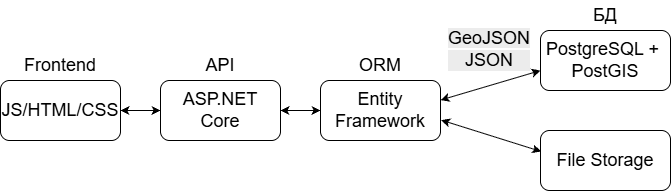
\includegraphics[width=0.95\textwidth]{../image/Stack.png}%
    \caption{Архитектурное взаимодействие компонентов веб-приложения.}
    \label{fig:architecture-components}
\end{figure}

\section{Архитектурные решения и принципы построения серверной части веб-приложения}

\subsection{Многоуровневая архитектура приложения}

Архитектура серверной части построена по многоуровневому принципу, при котором компоненты группируются по ответственности и взаимодействуют через явно определённые границы. Такой подход применяется для разделения задач представления, прикладных сценариев, предметной модели и инфраструктурных механизмов доступа к данным~\cite{sommerville2015software}. В рамках реализации выделяются следующие логические уровни:
\begin{itemize}
\item Presentation (уровень представления). Включает веб-интерфейс и серверные контроллеры API. На этом уровне выполняется приём запросов, разбор параметров и формирование ответов. Логика предметной области и операции с базой данных на уровне представления не размещаются;
\item Application (прикладной уровень). Содержит сценарии использования системы, определяющие последовательность действий для выполнения операций: получение данных на заданную дату, выборка объектов по фильтрам, формирование набора слоёв для отображения;
\item Domain (уровень предметной области). Определяет предметную область: основные сущности, их взаимосвязи и правила, которым должны соответствовать данные;
\item Infrastructure (инфраструктурный уровень). Включает механизмы работы с базой данных, реализацию репозиториев, настройку ORM и взаимодействие с файловым хранилищем.
\end{itemize}

В типовом потоке обработки пользовательский запрос поступает в контроллер API, далее управление передаётся прикладному сценарию, который использует предметные сущности и обращается к инфраструктурным интерфейсам доступа к данным. Результат преобразуется в структуру передачи данных и возвращается клиенту.

\subsection{Применение типовых архитектурных шаблонов}

Реализация серверной части опирается на типовые архитектурные шаблоны проектирования, применяемые в веб-приложениях на платформе .NET. Используемые шаблоны задают структуру взаимодействия компонентов и обеспечивают разделение ответственности между уровнями системы~\cite{fowler2002patterns,gamma1994design}.

Архитектурная модель строится на разделении компонентов по слоям: Presentation, Application, Domain и Infrastructure. Такое разграничение позволяет изолировать прикладную и предметную логику от деталей хранения данных и механизма взаимодействия по HTTP.

Компонентная структура серверной части и распределение основных элементов по слоям представлены на рисунке~\ref{fig:server-component-structure}. Данная схема используется для пояснения того, через какие уровни проходит запрос перед обращением к базе данных.

\begin{figure}[h]
    \centering
    \IfFileExists{../image/BackPattern.png}{%
        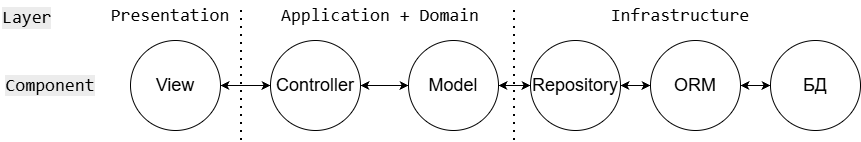
\includegraphics[width=0.95\textwidth]{../image/BackPattern.png}%
    }{%
        \fbox{\parbox[c][0.18\textheight][c]{0.9\textwidth}{\centering Временная заглушка для файла \texttt{BackPattern.png}.}}%
    }
    \caption{Компонентная структура серверной части и распределение по слоям.}
    \label{fig:server-component-structure}
\end{figure}

В рамках представленной структуры компоненты распределяются следующим образом:
\begin{itemize}
\item слой Presentation. Включает компонент View. Компонент View отвечает за формирование пользовательского интерфейса и передачу запросов к серверной части;
\item слой Application + Domain. Включает компонент Model, представляющий предметную модель системы, а также контроллеры Controller. На этом уровне располагаются сущности предметной области, их связи и правила обработки. Контроллеры принимают HTTP-запросы, выполняют их маршрутизацию, преобразование входных данных и передачу управления прикладному уровню, не выполняя прямого доступа к базе данных;
\item слой Infrastructure. Включает компоненты Repository, ORM и непосредственно базу данных. Репозитории реализуют интерфейсы доступа к данным и инкапсулируют операции выборки и сохранения. ORM Entity Framework обеспечивает отображение сущностей на реляционную структуру базы данных и формирование запросов. Хранение пространственных данных осуществляется с использованием возможностей PostGIS.
\end{itemize}

Маршрут прохождения запроса организован последовательно через указанные уровни. Пользовательское действие инициирует обращение к компоненту View, который формирует HTTP-запрос. Запрос поступает в Controller, где выполняется первичная обработка и передача управления прикладной логике. Далее обращение направляется к предметной модели, которая определяет правила выполнения операции. Для получения или изменения данных модель использует интерфейсы репозиториев. Репозиторий обращается к ORM, который формирует соответствующий запрос к базе данных. Полученный результат проходит обратный путь через слои Infrastructure, Application и Presentation и возвращается клиентской части.

Такое распределение компонентов обеспечивает:
\begin{itemize}
\item изоляцию предметной логики от механизма хранения данных;
\item независимость прикладного уровня от конкретной СУБД;
\item структурированное разграничение ответственности между уровнями;
\item возможность модификации инфраструктурных компонентов без изменения предметной модели.
\end{itemize}

MVC-подход в контексте Web API проявляется в том, что контроллеры выполняют функции уровня Presentation, принимая и обрабатывая HTTP-запросы. Модель отражает состояние предметной области и относится к уровням Application и Domain. Представление формируется на стороне клиента и также относится к уровню Presentation.

Шаблон Repository относится к инфраструктурному уровню и предоставляет унифицированный интерфейс доступа к данным. Он скрывает детали работы ORM и структуры таблиц, предоставляя прикладному уровню доступ к данным~\cite{fowler_repository}.

ORM и отображение сущностей реализуются средствами Entity Framework Core. Этот механизм обеспечивает сопоставление объектов программной модели с таблицами базы данных и отслеживание изменений сущностей. При работе с пространственными данными используются типы и функции PostGIS, что позволяет выполнять геометрические операции на уровне СУБД.

\section{Организация взаимодействия клиентской и серверной частей}

\subsection{Принципы REST-взаимодействия}

Связь между клиентской и серверной частями организуется в соответствии с архитектурным стилем REST. Сервер предоставляет набор ресурсов, соответствующих ключевым сущностям предметной области и прикладным операциям~\cite{fielding2000rest}.

Для выполнения операций используются стандартные HTTP-методы:
\begin{itemize}
\item GET --- получение наборов данных и деталей сущностей;
\item POST --- создание новых записей;
\item PUT/PATCH --- изменение существующих записей;
\item DELETE --- удаление записей.
\end{itemize}

Каждый запрос обрабатывается независимо: он содержит все данные, необходимые для выполнения операции, и не требует сохранения состояния сеанса на сервере. Для передачи данных применяется формат JSON, а для пространственных объектов --- GeoJSON. Ответы API формируются с использованием стандартных кодов состояния HTTP.

\subsection{Клиентская часть приложения и формат обмена данных}

Клиентская часть обеспечивает взаимодействие пользователя с системой: навигацию по данным, настройку отображаемых слоёв и работу с временной шкалой. Клиент формирует запросы к API и использует полученные ответы для построения визуальных представлений.

Для отображения пространственных объектов клиент получает данные в формате GeoJSON и преобразует их в элементы карты. Справочные данные и метаданные передаются в формате JSON. Связь файловых данных с сущностями системы реализуется через идентификаторы и метаданные, доступные через API~\cite{rfc7946}.

Для организации интерфейса может применяться CSS-фреймворк Bootstrap, предоставляющий набор готовых стилевых компонентов. Для картографической части фронтенда используется библиотека Leaflet, позволяющая отображать интерактивную карту, группировать пространственные объекты по слоям и обновлять их при изменении параметров запроса. Использование данных клиентских технологий рассматривается как средство ускорения разработки пользовательского интерфейса без изменения архитектурной структуры приложения.

\section{Проектирование структуры базы данных}

\subsection{Требования к БД и состав хранимой информации}

База данных веб-приложения «Палантир» является центральным компонентом системы, обеспечивающим хранение структурированной информации о военных конфликтах, их участниках, операциях, событиях и пространственных объектах. Поскольку приложение ориентировано на визуализацию данных, связанных с местом и временем, база данных должна поддерживать не только текстовые и справочные сведения, но и координаты, геометрические объекты и временные характеристики~\cite{silberschatz2019database}.

Предметная область проекта предполагает представление военных событий как пространственно-временного процесса. Поэтому в базе данных должны храниться сведения о войнах, театрах военных действий, операциях, сторонах конфликта, войсковых соединениях, событиях, положениях соединений и зонах контроля. Эти данные должны образовывать единую связанную структуру, пригодную для дальнейшей обработки серверной частью приложения.

Ключевыми требованиями к базе данных являются:
\begin{itemize}
    \item хранение структурированных и взаимосвязанных данных о конфликтах;
    \item поддержка иерархии «война --- театр военных действий --- операция»;
    \item хранение временных характеристик объектов и событий;
    \item поддержка пространственных типов для координат и зон контроля;
    \item обеспечение целостности данных с помощью первичных и внешних ключей;
    \item возможность последующего получения данных через серверное API.
\end{itemize}

Отдельное внимание должно уделяться хранению информации об участниках конфликта и войсковых соединениях. В системе необходимо различать сторону как самостоятельную сущность и её участие в конкретной войне или операции. Для соединений, в свою очередь, важно хранить не только основные сведения, но и их положение на карте в разные моменты времени~\cite{silberschatz2019database}.

С точки зрения картографической визуализации существенное значение имеют события и зоны контроля. События должны иметь дату, тип, описание и координату, а зоны контроля --- геометрию и временную привязку. Благодаря этому база данных может использоваться для отображения хода конфликта на карте и построения временной шкалы изменения обстановки~\cite{postgis_manual}.

Также необходимо учитывать, что исторические данные могут быть неполными или уточняться в процессе наполнения системы. Поэтому часть полей может допускать отсутствие значения, однако ключевые параметры, необходимые для идентификации и отображения данных, должны оставаться обязательными. Для пространственных данных важно предусмотреть и указание степени точности, поскольку положение объектов и границ в исторических источниках может быть приблизительным.

Таким образом, требования к базе данных веб-приложения «Палантир» определяются необходимостью хранения взаимосвязанных исторических, временных и пространственных данных. База данных должна обеспечивать целостное представление военных конфликтов, поддержку временной навигации, хранение геометрических объектов и возможность дальнейшего расширения структуры при развитии системы.

\subsection{Структура БД и реализация БД в PostgreSQL/PostGIS}

После определения требований к базе данных была разработана структура хранения данных для веб-приложения «Палантир». Основной задачей проектирования являлось создание такой модели, которая позволяла бы хранить сведения о военных конфликтах, их участниках, театрах военных действий, операциях, событиях, войсковых соединениях и пространственных объектах. При этом база данных должна поддерживать как реляционные связи между таблицами, так и хранение геометрических данных, необходимых для картографической визуализации.

На первоначальном этапе была сформирована логическая схема базы данных, позволившая определить основные сущности предметной области, их назначение и связи между ними. Логическая схема таблиц базы данных представлена на рисунке~\ref{fig:db-logical-schema}.

\begin{figure}[h]
    \centering
    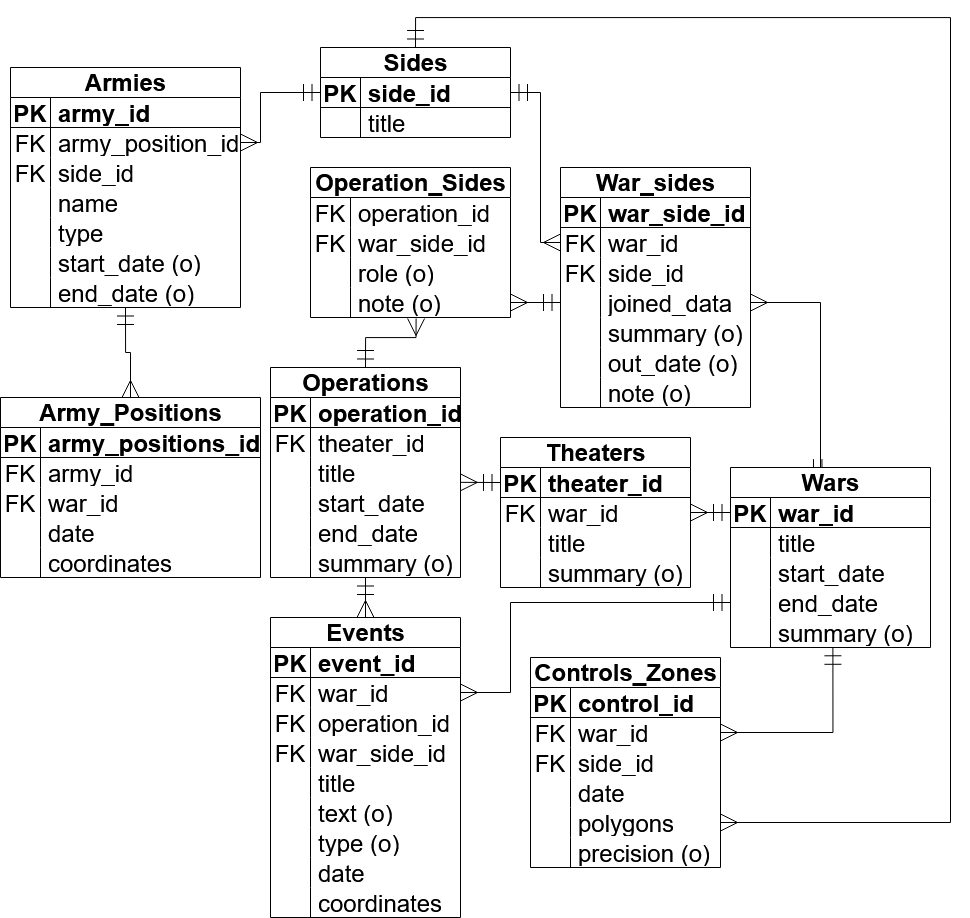
\includegraphics[width=0.72\textwidth]{../image/DB.png}
    \caption{Логическая схема таблиц базы данных веб-приложения «Палантир».}
    \label{fig:db-logical-schema}
\end{figure}

Реализация базы данных выполнена в PostgreSQL~\cite{postgresql_docs}. 
Для работы с пространственными объектами используется расширение PostGIS, которое добавляет поддержку геометрических типов данных. Это позволяет хранить не только текстовую и справочную информацию, но и координаты событий, положения войсковых соединений и полигоны зон контроля~\cite{postgis_manual}.

Использование PostGIS позволяет выполнять хранение и обработку пространственных объектов непосредственно на уровне базы данных, включая работу с точками, линиями, полигонами, пространственными индексами и запросами, применимыми в веб-картографических приложениях~\cite{obe_hsu_postgis_in_action}.

В структуре базы данных можно выделить несколько групп таблиц. Таблицы \texttt{wars}, \texttt{theaters} и \texttt{operations} задают иерархию конфликта: от войны к театрам военных действий и отдельным операциям. Таблицы \texttt{sides}, \texttt{war\_sides} и \texttt{operation\_sides} описывают участников конфликта и их роль в войнах и операциях. Таблицы \texttt{armies}, \texttt{army\_positions}, \texttt{events} и \texttt{control\_zones} содержат сведения о соединениях, их положении на карте, значимых событиях и контролируемых территориях. Такое разделение позволяет рассматривать данные как единую связанную модель и при этом сохранять логическую упорядоченность структуры~\cite{silberschatz2019database}.

Для краткого представления состава базы данных целесообразно обратиться к сводной таблице (см. таблицу~\ref{tab:db-main-tables}).

\begin{table}[H]
\caption{\label{tab:db-main-tables}Основные таблицы базы данных и их назначение}
\centering
\small
\begin{tabular}{|p{2.8cm}|p{12.2cm}|}
\hline
Таблица & Назначение \\
\hline
\texttt{wars} & Хранение общей информации о военных конфликтах \\
\hline
\texttt{theaters} & Хранение театров военных действий, относящихся к конкретной войне \\
\hline
\texttt{operations} & Хранение операций, проводимых в рамках театра военных действий \\
\hline
\texttt{sides} & Хранение справочной информации о сторонах конфликта \\
\hline
\texttt{war\_sides} & Связь сторон с конкретными войнами и хранение сведений об участии \\
\hline
\texttt{operation\_sides} & Связь сторон с конкретными операциями \\
\hline
\texttt{armies} & Хранение сведений о войсковых соединениях \\
\hline
\texttt{army\_positions} & Хранение положения соединений на карте по датам \\
\hline
\texttt{events} & Хранение событий, связанных с войной или операцией \\
\hline
\texttt{control\_zones} & Хранение зон контроля сторон конфликта \\
\hline
\end{tabular}
\end{table}

Ключевые связи в базе данных соответствуют логике предметной области. Война содержит театры военных действий, театр --- операции, а стороны конфликта связываются с войнами и операциями через промежуточные таблицы.~\cite{silberschatz2019database}.
Пространственная составляющая вынесена в таблицы \texttt{army\_positions} и \texttt{control\_zones}, что позволяет хранить изменение положения объектов и территорий во времени~\cite{postgresql_docs}. 
Полный SQL-скрипт создания базы данных приведён в приложении, а в основном тексте целесообразно показать только наиболее показательные фрагменты, один из которых представлен в листинге~\ref{code:db-key-tables}.

\begin{code}
\captionof{listing}{Фрагмент SQL-скрипта создания ключевых таблиц (полный код см. в приложении)}
\label{code:db-key-tables}
\vspace{-0.75cm}
\begin{minted}{sql}
CREATE EXTENSION IF NOT EXISTS postgis;
CREATE TABLE wars (
    war_id SERIAL PRIMARY KEY,
    title TEXT NOT NULL,
    start_date DATE NOT NULL,
    end_date DATE,
    summary TEXT
);
CREATE TABLE theaters (
    theater_id SERIAL PRIMARY KEY,
    war_id INT NOT NULL,
    title TEXT NOT NULL,
    summary TEXT,
    FOREIGN KEY (war_id) REFERENCES wars(war_id)
);
CREATE TABLE control_zones (
    control_id SERIAL PRIMARY KEY,
    war_id INT NOT NULL,
    war_side_id INT NOT NULL,
    date_control DATE NOT NULL,
    precision_control TEXT NOT NULL,
    geom geometry(MultiPolygon, 4326) NOT NULL,
    FOREIGN KEY (war_id) REFERENCES wars(war_id),
    FOREIGN KEY (war_side_id) REFERENCES war_sides(war_side_id)
);
\end{minted}
\end{code}

В приведённом фрагменте показаны базовая таблица военных конфликтов и иерархически связанная с ней таблица театров военных действий~\cite{postgresql_docs}. 
Таблица зон контроля демонстрирует использование пространственного типа \texttt{geometry(MultiPolygon, 4326)}~\cite{postgis_manual}. 
Такой набор примеров позволяет показать как реляционную структуру базы данных, так и её пространственное расширение без избыточного перечисления всех таблиц.

Для ускорения работы с данными в базе используются индексы. В контексте веб-приложения особенно важны индексы по внешним ключам, датам и геометрическим полям, поскольку они уменьшают время выборки связанных записей и ускоряют пространственные операции~\cite{postgresql_docs}. 
В качестве примера можно привести создание GiST-индекса для геометрии зон контроля, показанное в листинге~\ref{code:db-index-example}.

\begin{code}
\captionof{listing}{Пример создания пространственного индекса (полный код см. в приложении)}
\label{code:db-index-example}
\vspace{-0.75cm}
\begin{minted}{sql}
CREATE INDEX idx_control_zones_geom
    ON control_zones
    USING GIST(geom);
\end{minted}
\end{code}

Пространственный индекс ускоряет выполнение запросов к геометрическим объектам, включая выборку, фильтрацию и проверку пространственных отношений, что особенно важно для картографической визуализации данных и последующего пространственного анализа~\cite{postgis_manual}.

Таким образом, структура базы данных веб-приложения «Палантир» сочетает реляционную модель и возможности PostGIS. Она обеспечивает хранение связанных сущностей предметной области, поддержку временной навигации и работу с геометрическими объектами, создавая основу для дальнейшего доступа к данным из серверной части приложения.

\section{Реализация моделей и доступа к данным}

\subsection{Настройка Entity Framework Core и описание сущностей БД}

Для организации доступа серверной части веб-приложения «Палантир» к базе данных используется Entity Framework Core~\cite{efcore_overview}. 
Данная технология выполняет роль объектно-реляционного отображения и позволяет работать с таблицами базы данных через классы C\#, не формируя большинство SQL-запросов вручную~\cite{csharp_docs}. В рамках разрабатываемой системы это особенно важно, так как база данных содержит большое количество связанных сущностей: войны, театры военных действий, операции, стороны конфликта, армии, события и зоны контроля~\cite{smith_efcore_in_action}.

Для реализации системы была выбрана СУБД PostgreSQL с использованием расширения PostGIS, обеспечивающего поддержку пространственных типов данных. Подключение серверной части приложения к уже созданной структуре базы данных выполнено с применением подхода Database First, при котором Entity Framework Core формирует программную модель на основе существующей схемы БД~\cite{efcore_scaffolding}. 
В результате по структуре таблиц, первичным и внешним ключам, индексам и типам столбцов были получены Entity-классы базы данных, а также класс контекста \texttt{PalantirDbContext}~\cite{efcore_overview}.

Сгенерированные сущности были размещены в пространстве имён \texttt{Palantir.Domain.Models}, а сам \texttt{PalantirDbContext} --- в пространстве имён \texttt{Palantir.Infrastructure.Data}. Такой подход обеспечивает прямое соответствие между таблицами PostgreSQL/PostGIS и объектной моделью приложения. Сущности формируются на основе структуры БД и содержат свойства полей, навигационные связи и атрибуты сопоставления, автоматически отражающие схему данных~\cite{smith_efcore_in_action}.

Для системы «Палантир» важной особенностью является работа с пространственными объектами. На уровне базы данных она обеспечивается типами, предоставляемыми расширением PostGIS, а в приложении на языке C\# --- типами библиотеки NetTopologySuite~\cite{npgsql_postgis_nts}. 
Благодаря этому координаты событий, положения соединений и геометрия зон контроля единообразно представлены как в базе данных, так и в программном коде приложения~\cite{efcore_spatial}.

Центральным объектом взаимодействия с базой данных является \texttt{PalantirDbContext}. Он также был сгенерирован на основе существующей базы данных средствами Entity Framework Core и содержит наборы \texttt{DbSet}, соответствующие основным таблицам. Фрагмент данного класса приведён в листинге~\ref{code:db-context}.

\begin{code}
\captionof{listing}{Фрагмент класса \texttt{PalantirDbContext} (полный код см. в приложении)}
\label{code:db-context}
\vspace{-0.75cm}
\begin{minted}{csharp}
public partial class PalantirDbContext : DbContext {   
    public PalantirDbContext(DbContextOptions<PalantirDbContext> options) : base(options) {}
    public virtual DbSet<War> wars { get; set; }
    public virtual DbSet<Operation> operations { get; set; }
    public virtual DbSet<Event> events { get; set; }
    public virtual DbSet<ControlZone> control_zones { get; set; }
}
\end{minted}
\end{code}

Наборы \texttt{DbSet} обеспечивают доступ к таблицам базы данных через типизированные объекты и используются далее в репозиториях и сервисах приложения. Поскольку \texttt{PalantirDbContext} был сформирован по существующей структуре БД, его состав отражает актуальную схему данных и может быть расширен через механизм частичных классов без изменения сгенерированного кода напрямую~\cite{smith_efcore_in_action}.

Настройка подключения к базе данных выполняется в файле \texttt{Program.cs}, где приложение получает строку подключения из конфигурации~\cite{aspnet_configuration} и регистрирует \texttt{PalantirDbContext} в контейнере внедрения зависимостей~\cite{aspnet_docs}. Соответствующий фрагмент приведён в листинге~\ref{code:program-dbcontext}.

\begin{code}
\captionof{listing}{Регистрация контекста базы данных в \texttt{Program.cs}}
\label{code:program-dbcontext}
\vspace{-0.75cm}
\begin{minted}{csharp}
var connectionString =
    builder.Configuration.GetConnectionString(DatabaseSettings.ConnectionStringName)
    ?? throw new InvalidOperationException("Connection string not found");
builder.Services.AddDbContext<PalantirDbContext>(options =>
    options.UseNpgsql(
        connectionString,
        o => o.UseNetTopologySuite())
);
\end{minted}
\end{code}

Метод \texttt{UseNpgsql} указывает на использование PostgreSQL в качестве СУБД~\cite{npgsql_efcore_provider}. Дополнительный вызов \texttt{UseNetTopologySuite} обеспечивает корректную работу приложения с пространственными типами PostGIS, например \texttt{Point} и \texttt{MultiPolygon}~\cite{npgsql_postgis_nts}. 
В том же месте регистрируются и репозитории, через которые прикладной слой получает доступ к данным. Такая конфигурация завершает настройку компонентов доступа к базе данных и подготавливает переход к рассмотрению слоя Infrastructure.

\subsection{Реализация слоя Infrastructure для работы с БД}

Слой Infrastructure в серверной части приложения «Палантир» предназначен для реализации технических механизмов доступа к данным. В рамках данного слоя размещаются классы репозиториев, которые взаимодействуют с базой данных через \texttt{PalantirDbContext} и Entity Framework Core. За счёт этого прикладной уровень приложения не обращается к таблицам базы данных напрямую, а использует отдельные интерфейсы доступа к данным~\cite{lock_aspnet_core_in_action}.

Такой подход позволяет разделить прикладную логику и детали хранения информации. Слой Application может работать с абстракциями, не зная, каким именно образом данные извлекаются из PostgreSQL: через Entity Framework Core, SQL-запросы или иной механизм. Конкретная реализация доступа к данным находится в проекте \texttt{Palantir.Infrastructure}, а интерфейсы репозиториев вынесены в каталог \texttt{Palantir.Domain/Abstraction/Infrastructure/}. Это позволяет сохранить зависимость прикладной логики от интерфейсов, а не от конкретных инфраструктурных классов~\cite{lock_aspnet_core_in_action}.

Основным элементом слоя Infrastructure являются репозитории, отвечающие за доступ к данным по основным направлениям предметной области. Для каждой ключевой группы таблиц в проекте предусмотрены интерфейсы и их реализации, работающие через \texttt{PalantirDbContext}. Такая организация позволяет прикладному слою обращаться к данным через интерфейсы, не связывая бизнес-логику с конкретными средствами Entity Framework Core~\cite{fowler_repository}.

Репозитории имеют схожую структуру: они получают экземпляр \texttt{PalantirDbContext} через внедрение зависимостей, обращаются к соответствующим наборам \texttt{DbSet} и выполняют асинхронные операции чтения и изменения данных. В результате для прикладного слоя унифицируется работа с конфликтами, театрами военных действий, операциями, сторонами, событиями, позициями войск и зонами контроля.

Следует отметить, что интерфейсы репозиториев и классы их реализаций не относятся к автоматически сгенерированному коду Entity Framework Core. Если сущности базы данных и \texttt{PalantirDbContext} были получены на основе существующей схемы БД, то интерфейсы доступа к данным и соответствующие репозитории разрабатываются вручную. Это связано с тем, что именно они отражают выбранную архитектуру приложения и задают набор операций, доступных прикладному слою~\cite{efcore_scaffolding}.

В качестве примера можно рассмотреть интерфейс \texttt{IArmyRepository}, определяющий набор операций для работы с сущностью \texttt{Army}. Такой интерфейс фиксирует базовые операции получения, добавления, изменения и удаления данных, не раскрывая деталей конкретной реализации. Его фрагмент представлен в листинге~\ref{code:iarmy-repository}.

\begin{code}
\captionof{listing}{Интерфейс репозитория для работы с сущностью \texttt{Army}}
\label{code:iarmy-repository}
\vspace{-0.75cm}
\begin{minted}{csharp}
public interface IArmyRepository {
    Task<List<Army>> GetAllAsync();
    Task<Army?> GetByIdAsync(int id);
    Task AddAsync(Army army);
    Task UpdateAsync(Army army);
    Task DeleteAsync(int id);
}
\end{minted}
\end{code}

Наличие такого интерфейса позволяет прикладному уровню зависеть не от конкретного класса \texttt{ArmyRepository}, а от абстракции. Благодаря этому логика приложения не связывается напрямую с техническими деталями Entity Framework Core, а конкретную реализацию можно изменять без переработки кода сервисов и контроллеров~\cite{fowler_repository}.

Реализация интерфейса размещается в слое Infrastructure и использует \texttt{PalantirDbContext} для непосредственного обращения к базе данных. В отличие от Entity-классов, данный класс также создаётся разработчиком вручную и инкапсулирует конкретный способ выполнения операций над таблицей \texttt{armies}. Фрагмент реализации приведён в листинге~\ref{code:army-repository}.

\begin{code}
\captionof{listing}{Фрагмент реализации \texttt{ArmyRepository}}
\label{code:army-repository}
\vspace{-0.75cm}
\begin{minted}{csharp}
public class ArmyRepository : IArmyRepository {   
    private readonly PalantirDbContext _dbContext;
    public ArmyRepository(PalantirDbContext dbContext) {
        _dbContext = dbContext;
    }
    public async Task<List<Army>> GetAllAsync() =>
        await _dbContext.armies.ToListAsync<Army>();
    public async Task<Army?> GetByIdAsync(int id) =>
        await _dbContext.armies
            .FirstOrDefaultAsync(a => a.army_id == id);
    public async Task AddAsync(Army army) {
        await _dbContext.armies.AddAsync(army);
        await _dbContext.SaveChangesAsync();
    }
    public async Task UpdateAsync(Army army) {
        _dbContext.armies.Update(army);
        await _dbContext.SaveChangesAsync();
    }
    public async Task DeleteAsync(int id) {
        var army = await _dbContext.armies.FindAsync(id);
        if (army != null) {
            _dbContext.armies.Remove(army);
            await _dbContext.SaveChangesAsync();
        }
    }
}
\end{minted}
\end{code}

Из приведённого фрагмента видно, что класс \texttt{ArmyRepository} реализует интерфейс \texttt{IArmyRepository} и использует стандартные возможности Entity Framework Core для работы с данными. Метод \texttt{GetAllAsync} возвращает все записи из набора \texttt{armies}, \texttt{GetByIdAsync} выполняет поиск по идентификатору \texttt{army\_id}, а методы \texttt{AddAsync}, \texttt{UpdateAsync} и \texttt{DeleteAsync} изменяют данные и сохраняют результат вызовом \texttt{SaveChangesAsync}~\cite{smith_efcore_in_action}.

Отдельное значение имеют репозитории, работающие с пространственно-временными данными. При обращении к позициям войск и зонам контроля вместе с обычными атрибутами используются геометрические поля, поддерживаемые PostgreSQL/PostGIS и библиотекой NetTopologySuite~\cite{npgsql_postgis_nts}. 
По мере развития приложения такие классы могут быть дополнены методами выборки по дате, периоду времени, театру военных действий или операции, что важно для отображения исторических процессов на карте и временной шкале~\cite{efcore_spatial}.

Важной частью работы слоя Infrastructure является и его интеграция с контейнером внедрения зависимостей. Конкретные реализации репозиториев регистрируются в \texttt{Program.cs} как реализации соответствующих интерфейсов. Благодаря этому контроллеры и сервисы прикладного слоя получают зависимости через DI-контейнер, а не создают объекты репозиториев вручную. Такой способ организации соответствует многоуровневой архитектуре приложения и поддерживает изоляцию технических деталей доступа к данным внутри Infrastructure~\cite{aspnet_dependency_injection}.

Использование асинхронных методов является важной особенностью реализации репозиториев. Асинхронное выполнение операций обращения к базе данных позволяет серверному приложению эффективнее обрабатывать несколько запросов одновременно и не блокировать поток выполнения во время ожидания ответа от СУБД~\cite{csharp_docs}.

Таким образом, слой Infrastructure в проекте «Палантир» выполняет роль связующего уровня между прикладной моделью приложения и физической базой данных PostgreSQL/PostGIS. Репозитории инкапсулируют работу с Entity Framework Core и предоставляют прикладному уровню единый способ доступа к данным. В данной подглаве рассмотрены только основные и наиболее завершённые классы репозиториев, а полный исходный код реализаций и интерфейсов приведён в приложении к работе.


\subsection{Взаимодействие слоёв приложения при доступе к данным}

После настройки Entity Framework Core и описания слоя Infrastructure необходимо рассмотреть, каким образом запрос к данным проходит через уровни приложения. Для веб-приложения «Палантир» такой маршрут имеет принципиальное значение, поскольку система должна сохранять разделение ответственности между клиентским интерфейсом, серверным API, прикладной логикой, предметной моделью и механизмами хранения данных.

Типовой сценарий начинается с пользовательского действия в клиентской части. Пользователь выбирает конфликт, операцию, дату или слой карты, после чего клиентское приложение формирует HTTP-запрос к серверному API. Запрос поступает в слой Presentation, где находится API-контроллер. Контроллер отвечает за приём запроса, извлечение параметров, базовую проверку входных данных и формирование ответа, однако он не должен напрямую обращаться к таблицам базы данных или выполнять SQL-запросы. Такой подход соответствует многоуровневой архитектуре и снижает связанность между внешним интерфейсом API и техническими деталями хранения информации~\cite{lock_aspnet_core_in_action}.

После обработки входных параметров контроллер передаёт управление прикладной логике уровня Application. Данный уровень связывает пользовательский сценарий с операциями доступа к данным: например, получение списка армий, выборку событий по операции или подготовку данных для отображения на карте. При этом прикладной уровень должен зависеть не от конкретных классов Infrastructure, а от интерфейсов репозиториев. В проекте такие интерфейсы относятся к пространству имён \texttt{Palantir.Domain.Abstraction.Infrastructure}, что позволяет отделить правила предметной области и прикладные сценарии от конкретного способа работы с PostgreSQL/PostGIS.

Уровень Domain содержит сущности предметной области и абстракции, через которые остальные части приложения описывают работу с данными. К сущностям относятся модели из \texttt{Palantir.Domain.Models}, отражающие войны, операции, стороны конфликта, армии, события, позиции и зоны контроля. Уровень Infrastructure содержит реализации репозиториев, в том числе \texttt{ArmyRepository}, а также класс \texttt{PalantirDbContext}, размещённый в \texttt{Palantir.Infrastructure.Data}. Репозиторий использует \texttt{PalantirDbContext}, а контекст через Entity Framework Core и Npgsql обращается к PostgreSQL/PostGIS~\cite{npgsql_efcore_provider}.

Распределение ответственности между слоями приложения приведено в таблице~\ref{tab:data-access-layers}.

\begin{table}[H]
\caption{Распределение ролей слоёв при доступе к данным}
\label{tab:data-access-layers}
\centering
\small
\begin{tabular}{|p{2.5cm}|p{7.7cm}|p{4.8cm}|}
\hline
Слой & Назначение & Примеры компонентов \\
\hline
Presentation & Приём HTTP-запросов, извлечение параметров и формирование ответа клиентской части & API-контроллеры \\
\hline
Application & Выполнение прикладного сценария и обращение к данным через абстракции & Прикладные сценарии получения данных \\
\hline
Domain & Описание сущностей предметной области и интерфейсов доступа к данным & \texttt{Palantir.Domain.Models}, интерфейсы репозиториев \\
\hline
Infrastructure & Реализация технического доступа к базе данных и скрытие деталей хранения & \texttt{PalantirDbContext}, репозитории, \texttt{ArmyRepository} \\
\hline
\end{tabular}
\end{table}

После получения данных из базы репозиторий возвращает результат прикладному уровню. Далее данные могут быть преобразованы в DTO или response-модели, предназначенные для передачи клиентской части. Такое преобразование необходимо потому, что структура внутренней модели базы данных не всегда должна совпадать со структурой ответа API. Например, для клиентского интерфейса может быть важен только ограниченный набор полей, а для карты требуется представление пространственного объекта в формате GeoJSON~\cite{rfc7946}.

Обратный путь результата проходит через те же архитектурные границы. Infrastructure возвращает данные прикладному уровню, Application подготавливает ответ в соответствии со сценарием использования, Presentation формирует HTTP-ответ, а клиентская часть получает данные в формате JSON или GeoJSON. Таким образом, слой Infrastructure скрывает технические детали хранения данных, слой Domain задаёт сущности и абстракции, слой Application связывает пользовательские сценарии с доступом к данным, а слой Presentation выполняет роль внешней точки взаимодействия с клиентом.

Описанная схема показывает общий принцип организации доступа к данным в веб-приложении «Палантир». После рассмотрения маршрута запроса через уровни приложения целесообразно перейти к примерам запросов к базе данных через Entity Framework Core, поскольку именно они демонстрируют практический механизм получения и изменения данных в слое Infrastructure.

\subsection{Примеры запросов к БД через EF Core}

Entity Framework Core используется в серверной части приложения как основной механизм объектно-реляционного отображения. Его применение позволяет выполнять запросы к PostgreSQL через типизированные объекты C\# и выражения LINQ, не формируя большинство SQL-запросов вручную~\cite{efcore_overview}. При выполнении запроса EF Core преобразует LINQ-выражение в SQL-команду, отправляет её в СУБД через провайдер Npgsql и возвращает результат в виде объектов предметной модели.

В качестве типового примера можно рассмотреть уже приведённый в листинге~\ref{code:army-repository} фрагмент репозитория \texttt{ArmyRepository}. Метод \texttt{GetAllAsync} обращается к набору \texttt{DbSet} \texttt{armies} и получает список всех записей с помощью \texttt{ToListAsync}. Метод \texttt{GetByIdAsync} использует \texttt{FirstOrDefaultAsync} и условие по идентификатору \texttt{army\_id}. В обоих случаях запросы описываются средствами LINQ, а конкретный SQL-код формируется Entity Framework Core автоматически.

Для операций изменения данных репозиторий использует методы \texttt{AddAsync}, \texttt{Update} и \texttt{Remove}. После добавления, изменения или удаления объекта вызывается \texttt{SaveChangesAsync}, который фиксирует накопленные изменения в базе данных. Асинхронная форма этих операций позволяет серверному приложению не блокировать поток выполнения во время ожидания ответа от СУБД, что особенно важно для веб-приложения, одновременно обрабатывающего несколько HTTP-запросов~\cite{csharp_docs}.

При подготовке ответов для API данные, полученные через репозиторий, целесообразно преобразовывать в отдельные response-модели. Такой подход позволяет не возвращать клиентской части внутренние Entity-классы напрямую и контролировать структуру ответа. В качестве типового структурного примера можно рассмотреть преобразование сущности армии в краткую модель ответа, приведённое в листинге~\ref{code:army-response-example}.

\begin{code}
\captionof{listing}{Пример подготовки краткой response-модели для API}
\label{code:army-response-example}
\vspace{-0.75cm}
\begin{minted}{csharp}
var army = await armyRepository.GetByIdAsync(id);
if (army == null) {
    return null;
}
var response = new {
    Id = army.army_id,
    Title = army.title,
    Type = army.type
};
\end{minted}
\end{code}

Данный фрагмент не описывает отдельный обязательный класс проекта, а показывает общий принцип подготовки ответа: из сущности выбираются только те поля, которые необходимы клиентскому приложению. Такой подход удобен для справочных данных, отображаемых в списках, карточках объектов или панели сведений о выбранном соединении.

Для пространственно-временных данных принцип остаётся тем же, однако в запросах дополнительно учитываются дата, принадлежность к операции или стороне конфликта, а также геометрическое поле. Пространственные типы в приложении должны быть совместимы с PostGIS и NetTopologySuite, что позволяет хранить и получать точки, линии и полигоны без ручного преобразования координат~\cite{npgsql_postgis_nts}. Такая организация соответствует практическому применению пространственных типов и запросов PostGIS в веб-картографических приложениях~\cite{obe_hsu_postgis_in_action}. В качестве типового примера можно рассмотреть выборку зон контроля на заданную дату, показанную в листинге~\ref{code:control-zone-query-example}.

\begin{code}
\captionof{listing}{Типовой пример выборки пространственных данных по дате}
\label{code:control-zone-query-example}
\vspace{-0.75cm}
\begin{minted}{csharp}
var zones = await dbContext.control_zones
    .Where(zone => zone.date_control <= selectedDate)
    .ToListAsync();
\end{minted}
\end{code}

Пример демонстрирует подход к выборке объектов, связанных с временной привязкой. Полученные записи могут использоваться прикладным уровнем для подготовки ответа API, а геометрия зоны контроля --- для последующего формирования GeoJSON-структуры. В реальной реализации конкретные условия выборки могут уточняться с учётом войны, операции, стороны конфликта и требуемого временного среза.

Таким образом, запросы через Entity Framework Core позволяют связать реляционную и пространственную структуру PostgreSQL/PostGIS с объектной моделью серверного приложения. Репозитории инкапсулируют эти операции, а прикладной уровень получает данные в форме, пригодной для дальнейшей передачи через серверное API.

\section{Реализация серверного API}

Для взаимодействия клиентской части веб-приложения с серверной частью реализуется программный интерфейс API. Серверное API предназначено для приёма запросов от клиента, обработки переданных параметров, обращения к прикладной логике и возвращения данных в формате, пригодном для дальнейшего отображения в пользовательском интерфейсе~\cite{aspnet_docs}.

В рамках проекта «Палантир» API используется для работы с основными сущностями предметной области: войнами, сторонами конфликта, зонами контроля, операциями и другими объектами, связанными с отображением пространственно-временных данных. Клиентская часть отправляет HTTP-запросы к серверу, после чего сервер возвращает структурированный ответ, содержащий необходимые данные.

Для передачи данных между клиентом и сервером используются специальные классы-контракты. Они разделяются на два основных типа:
\begin{itemize}
\item \texttt{Request} --- модели входных данных, которые клиент передаёт серверу;
\item \texttt{Response} --- модели выходных данных, которые сервер возвращает клиенту.
\end{itemize}

Такое разделение позволяет не передавать клиенту внутренние сущности базы данных напрямую, а использовать отдельные структуры, предназначенные именно для обмена данными через API. Это повышает гибкость системы, упрощает сопровождение кода и позволяет изменять внутреннюю структуру базы данных без необходимости менять формат взаимодействия с клиентской частью.

Примером входной модели является класс \texttt{WarRequest}, предназначенный для передачи данных при создании или изменении записи о войне. Фрагмент модели представлен в листинге~\ref{code:war-request-api}.

\begin{code}
\captionof{listing}{Модель запроса \texttt{WarRequest}}
\label{code:war-request-api}
\vspace{-0.75cm}
\begin{minted}{csharp}
public record class WarRequest(
    string Title,
    DateOnly StartDate,
    DateOnly? EndDate,
    string? Summary
);
\end{minted}
\end{code}

Данная модель содержит название войны, дату начала, необязательную дату окончания и краткое описание. Использование типа \texttt{DateOnly} позволяет явно указать, что в данной модели важна именно календарная дата, а не точное время суток. Поля \texttt{EndDate} и \texttt{Summary} сделаны необязательными, так как для некоторых конфликтов дата окончания может быть неизвестна или описание может отсутствовать на момент создания записи.

Соответствующая модель ответа \texttt{WarResponse} дополнительно содержит идентификатор записи. Её структура приведена в листинге~\ref{code:war-response-api}.

\begin{code}
\captionof{listing}{Модель ответа \texttt{WarResponse}}
\label{code:war-response-api}
\vspace{-0.75cm}
\begin{minted}{csharp}
public record class WarResponse(
    int Id,
    string Title,
    DateOnly StartDate,
    DateOnly? EndDate,
    string? Summary
);
\end{minted}
\end{code}

Наличие поля \texttt{Id} в ответе необходимо для дальнейшего обращения к конкретной записи со стороны клиентского приложения. Например, после создания новой войны клиент может использовать полученный идентификатор для загрузки связанных с ней сторон, операций, событий или зон контроля.

Пример HTTP-запроса на создание записи о войне представлен в листинге~\ref{code:war-create-request-api}.

\begin{code}
\captionof{listing}{Пример запроса на создание записи о войне}
\label{code:war-create-request-api}
\vspace{-0.75cm}
\begin{minted}{json}
POST /api/wars
Content-Type: application/json {
  "title": "Великая Отечественная война",
  "startDate": "1941-06-22",
  "endDate": "1945-05-09",
  "summary": "Военный конфликт между СССР и странами нацистского блока в рамках Второй мировой войны."
}
\end{minted}
\end{code}

После обработки запроса сервер может вернуть ответ, приведённый в листинге~\ref{code:war-create-response-api}.

\begin{code}
\captionof{listing}{Пример ответа после создания записи о войне}
\label{code:war-create-response-api}
\vspace{-0.75cm}
\begin{minted}{http}
HTTP/1.1 201 Created
Content-Type: application/json {
  "id": 1,
  "title": "Великая Отечественная война",
  "startDate": "1941-06-22",
  "endDate": "1945-05-09",
  "summary": "Военный конфликт между СССР и странами нацистского блока в рамках Второй мировой войны."
}
\end{minted}
\end{code}

Таким образом, клиент передаёт серверу только данные, необходимые для создания записи, а сервер возвращает уже сформированный объект с присвоенным идентификатором.

Отдельное значение в системе имеют модели, связанные с зонами контроля. Зона контроля представляет собой пространственный объект, который показывает территорию, контролируемую определённой стороной конфликта на конкретную дату. Для создания такой записи используется модель \texttt{CreateControlZoneRequest}, показанная в листинге~\ref{code:create-control-zone-request-api}.

\begin{code}
\captionof{listing}{Модель запроса \texttt{CreateControlZoneRequest}}
\label{code:create-control-zone-request-api}
\vspace{-0.75cm}
\begin{minted}{csharp}
public record class CreateControlZoneRequest(
    int WarId,
    int WarSideId,
    DateOnly DateControl,
    string PrecisionControl,
    MultiPolygon Geom
);
\end{minted}
\end{code}

Данная модель содержит идентификатор войны, идентификатор стороны конфликта, дату фиксации зоны контроля, описание точности данных и геометрию объекта. Поле \texttt{Geom} имеет тип \texttt{MultiPolygon}, что позволяет хранить сложные полигональные объекты, состоящие из нескольких областей. Это важно для отображения зон контроля, так как территория, находящаяся под контролем одной стороны, может быть не сплошной, а состоять из нескольких отдельных участков~\cite{npgsql_postgis_nts}.

Поле \texttt{PrecisionControl} используется для указания степени точности пространственных данных. Например, зона контроля может быть получена на основе исторической карты, приблизительной реконструкции или другого источника, не всегда позволяющего определить границы абсолютно точно. Такое поле позволяет учитывать специфику исторических данных, где пространственная информация может иметь различную степень достоверности.

Для обновления зоны контроля используется отдельная модель \texttt{UpdateControlZoneRequest}, представленная в листинге~\ref{code:update-control-zone-request-api}.

\begin{code}
\captionof{listing}{Модель запроса \texttt{UpdateControlZoneRequest}}
\label{code:update-control-zone-request-api}
\vspace{-0.75cm}
\begin{minted}{csharp}
public record class UpdateControlZoneRequest(
    string PrecisionControl,
    MultiPolygon Geom
);
\end{minted}
\end{code}

В данной модели отсутствуют поля \texttt{WarId}, \texttt{WarSideId} и \texttt{DateControl}, так как при изменении уже существующей зоны контроля обычно корректируются именно геометрия и характеристика точности, а принадлежность к войне, стороне конфликта и дате остаётся неизменной. Это позволяет ограничить набор изменяемых данных и снизить вероятность случайного нарушения связей между сущностями.

Модель ответа для зоны контроля содержит идентификатор зоны контроля, связь с войной и стороной конфликта, дату, описание точности и геометрию. Такой ответ может использоваться клиентской частью для отображения полигона на карте. Структура модели приведена в листинге~\ref{code:control-zone-response-api}.

\begin{code}
\captionof{listing}{Модель ответа \texttt{ControlZoneResponse}}
\label{code:control-zone-response-api}
\vspace{-0.75cm}
\begin{minted}{csharp}
public record class ControlZoneResponse(
    int Id,
    int WarId,
    int WarSideId,
    DateOnly DateControl,
    string PrecisionControl,
    MultiPolygon Geom
);
\end{minted}
\end{code}

Пример запроса на создание зоны контроля представлен в листинге~\ref{code:control-zone-create-request-api}.

\begin{code}
\captionof{listing}{Пример запроса на создание зоны контроля}
\label{code:control-zone-create-request-api}
\vspace{-0.75cm}
\begin{minted}{json}
POST /api/control-zones
Content-Type: application/json {
  "warId": 1,
  "warSideId": 2,
  "dateControl": "1943-07-12",
  "precisionControl": "Граница зоны контроля построена по исторической карте и имеет приблизительный характер.",
  "geom": {
    "type": "MultiPolygon",
    "coordinates": [[[
          [36.10, 51.20],
          [36.40, 51.25],
          [36.35, 51.05],
          [36.10, 51.20]]]]}
}
\end{minted}
\end{code}

После успешного создания сервер возвращает данные созданной зоны контроля. Пример ответа приведён в листинге~\ref{code:control-zone-create-response-api}.

\begin{code}
\captionof{listing}{Пример ответа после создания зоны контроля}
\label{code:control-zone-create-response-api}
\vspace{-0.75cm}
\begin{minted}{http}
HTTP/1.1 201 Created
Content-Type: application/json {
  "id": 15,
  "warId": 1,
  "warSideId": 2,
  "dateControl": "1943-07-12",
  "precisionControl": "Граница зоны контроля построена по исторической карте и имеет приблизительный характер.",
  "geom": {
    "type": "MultiPolygon",
    "coordinates": [[[
          [36.10, 51.20],
          [36.40, 51.25],
          [36.35, 51.05],
          [36.10, 51.20]]]]}
}
\end{minted}
\end{code}

Пример изменения зоны контроля представлен в листинге~\ref{code:control-zone-update-request-api}.

\begin{code}
\captionof{listing}{Пример запроса на изменение зоны контроля}
\label{code:control-zone-update-request-api}
\vspace{-0.75cm}
\begin{minted}{json}
PUT /api/control-zones/15
Content-Type: application/json {
  "precisionControl": "Геометрия уточнена на основе дополнительного картографического источника.",
  "geom": {
    "type": "MultiPolygon",
    "coordinates": [[[
          [36.12, 51.22],
          [36.42, 51.27],
          [36.36, 51.04],
          [36.12, 51.22]]]]}
}
\end{minted}
\end{code}

В результате сервер обновляет геометрию и характеристику точности для существующей записи. Такой подход особенно важен для системы «Палантир», поскольку пространственные данные о боевых действиях могут уточняться по мере добавления новых источников.

Использование отдельных моделей запросов и ответов позволяет явно определить границы взаимодействия между клиентом и сервером. Клиентская часть не работает напрямую с таблицами базы данных, а взаимодействует с API через заранее определённые контракты. Серверная часть, в свою очередь, принимает входные данные, выполняет проверку, обращается к базе данных через слой инфраструктуры и возвращает результат в виде ответа.

Таким образом, реализация серверного API обеспечивает связь между пользовательским интерфейсом, прикладной логикой и базой данных. API выступает промежуточным уровнем, который принимает HTTP-запросы, преобразует входные данные в структуры приложения, выполняет необходимые операции и возвращает клиенту данные в унифицированном формате. Это соответствует выбранной клиент-серверной архитектуре и обеспечивает возможность дальнейшего расширения системы за счёт добавления новых маршрутов, моделей запросов и моделей ответов.

\chapter{РЕАЛИЗАЦИЯ КЛИЕНТСКОЙ ЧАСТИ, ТЕСТИРОВАНИЕ И РАЗВЁРТЫВАНИЕ ВЕБ-ПРИЛОЖЕНИЯ}

Третья глава посвящена реализации клиентской части веб-приложения «Палантир», описанию картографической визуализации пространственно-временных данных, а также проверке работоспособности основных компонентов и подготовке системы к эксплуатации в составе серверной среды. Если в предыдущей главе основное внимание уделялось проектированию архитектуры, базы данных, слоя доступа к базе данных и серверного API, то в рамках данной главы рассматриваются вопросы фронтенда, интеграционного тестирования, подготовки к развёртыванию и проверки приложения после размещения~\cite{sommerville2015software}.

Поскольку разрабатываемая система предназначена для хранения, обработки и визуализации данных об исторических военных конфликтах, клиентская часть должна обеспечивать наглядное представление пространственно-временных данных на карте и корректное взаимодействие с серверным API. Практическая значимость данного этапа заключается в подтверждении того, что разработанные компоненты способны функционировать как части единой веб-информационной системы, объединяющей интерфейс пользователя, серверную логику и базу данных.

\section{Реализация клиентской части веб-приложения}

Клиентская часть веб-приложения «Палантир» предназначена для взаимодействия пользователя с системой и представления данных, полученных от серверного API. Её основная роль заключается не в хранении или обработке предметной информации, а в обеспечении навигации, отображении сведений и визуализации пространственно-временных объектов на карте.

В составе клиентского уровня предусматриваются элементы интерфейса, необходимые для работы с историческими военными конфликтами: область карты, панель выбора отображаемых слоёв, элементы временной навигации, средства выбора войны или операции, а также информационная область для отображения сведений о выбранном объекте. Данные для этих элементов поступают от серверной части в форматах JSON и GeoJSON. JSON используется для обычных справочных сведений, а GeoJSON --- для объектов, имеющих координаты или геометрию.

Клиентский уровень формирует запросы к API на основании действий пользователя. При выборе конфликта, операции, даты или слоя отображения клиент отправляет HTTP-запрос с соответствующими параметрами. Полученный ответ используется для обновления интерфейса: списков, карточек, элементов карты и состава отображаемых слоёв. Такой подход позволяет отделить визуальное представление от серверной логики и базы данных.

Основные элементы клиентской части и их связь с серверным API представлены в таблице~\ref{tab:client-elements}.

\begin{table}[H]
\caption{Элементы клиентской части веб-приложения}
\label{tab:client-elements}
\centering
\small
\begin{tabular}{|p{3.5cm}|p{5.4cm}|p{4.7cm}|}
\hline
Элемент клиентской части & Назначение & Связь с серверным API \\
\hline
Карта & Отображение событий, позиций соединений и зон контроля & Получение пространственных объектов в GeoJSON \\
\hline
Временная шкала & Выбор даты или периода для анализа хода конфликта & Передача временных параметров в запросах \\
\hline
Панель слоёв & Управление отображением армий, событий и зон контроля & Запрос данных по выбранным типам объектов \\
\hline
Информационная карточка & Отображение сведений о выбранном объекте & Получение детальной информации по идентификатору \\
\hline
\end{tabular}
\end{table}

Для реализации интерфейса могут использоваться HTML, CSS и JavaScript. CSS-фреймворк Bootstrap, уже рассматриваемый при описании клиентской части, может применяться для унификации внешнего вида элементов управления и ускорения разработки интерфейсных компонентов. Для фронтенд-реализации интерактивной карты дополнительно применяется библиотека Leaflet, обеспечивающая работу с картографической подложкой, маркерами, полигонами, полилиниями и группами слоёв. При этом использование Bootstrap и Leaflet не влияет на архитектурное разделение системы: клиентская часть остаётся потребителем API и не выполняет прямой доступ к базе данных.

Особое значение для клиентской части имеет корректная интерпретация данных, полученных от сервера. Справочные JSON-ответы используются для заполнения списков и информационных блоков, а GeoJSON-объекты преобразуются в элементы карты. При изменении временного параметра или набора слоёв клиентская часть должна обновлять отображаемые объекты, чтобы карта отражала выбранный временной срез исторического процесса.

Таким образом, клиентская часть выполняет роль визуального и навигационного уровня веб-приложения. Она связывает действия пользователя с серверным API и обеспечивает представление данных в форме, пригодной для анализа исторических военных событий. Наиболее важной частью данного представления является картографическая визуализация пространственно-временных данных.

\section{Реализация картографической визуализации операции}

Одной из ключевых частей клиентской стороны веб-информационной системы «Палантир» является модуль картографической визуализации операции. Данный модуль предназначен для отображения пространственных объектов, связанных с выбранной боевой операцией: событий, войсковых соединений, зон контроля и линии фронта. Реализация выполнена средствами HTML, JavaScript и библиотеки Leaflet, которая используется для создания интерактивной карты в веб-интерфейсе.

Страница карты операции содержит две основные области: боковую панель управления и область отображения карты. В боковой панели размещаются элементы навигации, сведения об операции, переключатели картографических слоёв, элемент временной шкалы, а также список объектов, отображаемых на карте. Основная область страницы предназначена непосредственно для вывода интерактивной карты. В HTML-разметке для этого используется контейнер с идентификатором \texttt{map}, к которому в дальнейшем подключается логика библиотеки Leaflet.

Подключение функциональной части страницы выполняется через JavaScript-файл \texttt{map-page.js}. В нём сосредоточена основная логика работы карты: получение параметров страницы, инициализация картографической подложки, загрузка сведений об операции, создание слоёв, добавление объектов на карту, управление отображением слоёв и навигация по объектам.

При открытии страницы карта получает идентификатор операции из строки запроса. Например, страница может быть открыта в формате, приведённом в листинге~\ref{code:map-url-example}.

\begin{code}
\captionof{listing}{Пример адреса страницы карты операции}
\label{code:map-url-example}
\vspace{-0.75cm}
\begin{minted}{text}
/map.html?operationId=1
\end{minted}
\end{code}

Для получения параметра используется функция, основанная на объекте \texttt{URLSearchParams}. Её фрагмент показан в листинге~\ref{code:map-query-param}.

\begin{code}
\captionof{listing}{Получение параметра из строки запроса}
\label{code:map-query-param}
\vspace{-0.75cm}
\begin{minted}{javascript}
function getQueryParam(name) {
    return new URLSearchParams(window.location.search).get(name);
}
\end{minted}
\end{code}

Полученный идентификатор сохраняется во внутреннем состоянии страницы. Это позволяет использовать одну страницу карты для разных операций, так как конкретная операция определяется не отдельным HTML-файлом, а параметром \texttt{operationId}.

Для хранения текущего состояния страницы используется объект \texttt{pageState}, структура которого представлена в листинге~\ref{code:map-page-state}.

\begin{code}
\captionof{listing}{Объект состояния страницы карты}
\label{code:map-page-state}
\vspace{-0.75cm}
\begin{minted}{javascript}
const pageState = {
    operationId: getQueryParam("operationId"),
    operation: null,
    featureLayers: []
};
\end{minted}
\end{code}

Поле \texttt{operationId} хранит идентификатор выбранной операции, поле \texttt{operation} предназначено для хранения данных операции, полученных от серверного API, а массив \texttt{featureLayers} используется для сохранения всех добавленных на карту объектов. Наличие общего списка объектов позволяет выполнять автоматическое масштабирование карты по всем отображаемым элементам.

Инициализация карты выполняется с помощью библиотеки Leaflet. Для карты задаются координаты центра по умолчанию и начальный уровень масштабирования, как показано в листинге~\ref{code:leaflet-map-init}.

\begin{code}
\captionof{listing}{Инициализация карты Leaflet}
\label{code:leaflet-map-init}
\vspace{-0.75cm}
\begin{minted}{javascript}
const DEFAULT_CENTER = [51.75, 36.19];
const DEFAULT_ZOOM = 7;

const map = L.map("map", {
    zoomControl: true,
    attributionControl: true
}).setView(DEFAULT_CENTER, DEFAULT_ZOOM);
\end{minted}
\end{code}

После создания объекта карты подключается картографическая подложка. В качестве источника тайлов используется сервис Яндекс.Карт. API-ключ вынесен в отдельный конфигурационный файл, что позволяет отделить настройки доступа к внешнему картографическому сервису от основной логики страницы. Пример подключения тайлового слоя приведён в листинге~\ref{code:leaflet-yandex-tiles}.

\begin{code}
\captionof{listing}{Подключение картографической подложки}
\label{code:leaflet-yandex-tiles}
\vspace{-0.75cm}
\begin{minted}[mathescape=false]{javascript}
const yandexTilesApiKey = window.PALANTIR_MAP_CONFIG?.YANDEX_TILES_API_KEY;
const yandexTileUrl =
    "https://tiles.api-maps.yandex.ru/v1/tiles/" +
    "?x={x}&y={y}&z={z}&lang=ru_RU&l=map" +
    `&projection=web_mercator&apikey=${yandexTilesApiKey}`;

L.tileLayer(yandexTileUrl, {
    maxZoom: 19,
    tileSize: 256
}).addTo(map);
\end{minted}
\end{code}

Такой подход обеспечивает возможность централизованного изменения параметров подключения к картографическому сервису без изменения основного кода визуализации.

Для отображения разных типов данных на карте используются отдельные логические слои. Это позволяет независимо управлять видимостью событий, зон контроля, войсковых соединений и линии фронта. Структура слоёв приведена в листинге~\ref{code:leaflet-layer-groups}.

\begin{code}
\captionof{listing}{Создание логических слоёв карты}
\label{code:leaflet-layer-groups}
\vspace{-0.75cm}
\begin{minted}{javascript}
const mapLayers = {
    events: L.layerGroup().addTo(map),
    controlZones: L.layerGroup().addTo(map),
    armies: L.layerGroup().addTo(map),
    frontLines: L.layerGroup().addTo(map)
};
\end{minted}
\end{code}

Каждый слой представляет собой объект \texttt{L.layerGroup}. В него добавляются только объекты соответствующего типа. Например, события операции помещаются в слой \texttt{events}, зоны контроля --- в \texttt{controlZones}, войсковые соединения --- в \texttt{armies}, а линия фронта --- в \texttt{frontLines}. Такое разделение упрощает управление картой и делает интерфейс более гибким для пользователя.

Переключение слоёв реализуется через элементы управления в боковой панели. Для каждого переключателя назначается обработчик события \texttt{change}. Если переключатель включён, слой добавляется на карту, если выключен --- удаляется. Универсальная функция обработки переключателя представлена в листинге~\ref{code:leaflet-layer-toggle}.

\begin{code}
\captionof{listing}{Управление видимостью слоя карты}
\label{code:leaflet-layer-toggle}
\vspace{-0.75cm}
\begin{minted}{javascript}
function bindLayerToggle(checkbox, layer) {
    checkbox.addEventListener("change", function () {
        if (checkbox.checked) {
            layer.addTo(map);
        } else {
            map.removeLayer(layer);
        }
    });
}
\end{minted}
\end{code}

Данная функция является универсальной и используется для всех слоёв карты. Благодаря этому код не дублируется для каждого типа объектов, а управление слоями выполняется единообразно.

Загрузка сведений об операции выполняется асинхронно. После получения идентификатора операции клиентская часть отправляет запрос к серверному API. Полученные данные сохраняются в состоянии страницы и используются для заполнения информационного блока. Общая структура такой функции приведена в листинге~\ref{code:map-load-operation}.

\begin{code}
\captionof{listing}{Загрузка сведений об операции}
\label{code:map-load-operation}
\vspace{-0.75cm}
\begin{minted}{javascript}
async function loadOperation(operationId) {
    const operation = await fetchOperation(operationId);
    pageState.operation = operation;

    renderOperationInfo(operation);
    setMapCenterFromOperation(operation);
}
\end{minted}
\end{code}

Функция \texttt{renderOperationInfo} отвечает за вывод основной информации об операции: идентификатора, названия, дат начала и окончания, а также описания. При формировании HTML-содержимого используется функция экранирования данных, что снижает риск некорректной вставки пользовательского или внешнего текста в разметку страницы.

Если в данных операции присутствуют координаты центра, карта автоматически перемещается к соответствующей области. Для этого используется функция \texttt{setMapCenterFromOperation}, показанная в листинге~\ref{code:map-center-from-operation}.

\begin{code}
\captionof{listing}{Установка центра карты по данным операции}
\label{code:map-center-from-operation}
\vspace{-0.75cm}
\begin{minted}{javascript}
function setMapCenterFromOperation(operation) {
    const lat = operation.centerLat ?? operation.latitude ?? operation.lat;
    const lng = operation.centerLng ?? operation.longitude ?? operation.lng;

    if (isValidCoordinate(lat) && isValidCoordinate(lng)) {
        map.setView([Number(lat), Number(lng)], operation.zoom ?? DEFAULT_ZOOM);
    }
}
\end{minted}
\end{code}

В данном фрагменте предусмотрена проверка корректности координат. Это позволяет избежать ошибки при попытке переместить карту к неопределённым или некорректным значениям.

Отображение объектов на карте выполняется с использованием разных типов графических элементов Leaflet. События и войсковые соединения отображаются маркерами, линия фронта --- полилинией, зоны контроля --- полигонами. Для каждого объекта создаётся всплывающее окно с краткой информацией.

Пример добавления события на карту приведён в листинге~\ref{code:map-event-marker}.

\begin{code}
\captionof{listing}{Добавление события на карту}
\label{code:map-event-marker}
\vspace{-0.75cm}
\begin{minted}[mathescape=false]{javascript}
function addEventMarker(event) {
    const marker = L.marker([event.lat, event.lng], { icon: eventIcon })
        .bindPopup(`
            <strong>${escapeHtml(event.title)}</strong><br>
            <span>${escapeHtml(formatDate(event.date))}</span><br>
            <span>${escapeHtml(event.description)}</span>
        `);

    marker.addTo(mapLayers.events);
    pageState.featureLayers.push(marker);
}
\end{minted}
\end{code}

В данном случае маркер создаётся по координатам события. К нему привязывается всплывающее окно, содержащее название события, дату и описание. После создания маркер добавляется в слой событий и сохраняется в массиве \texttt{featureLayers}.

Войсковые соединения отображаются схожим образом, однако помещаются в отдельный слой. Пример такой функции приведён в листинге~\ref{code:map-army-marker}.

\begin{code}
\captionof{listing}{Добавление войскового соединения на карту}
\label{code:map-army-marker}
\vspace{-0.75cm}
\begin{minted}[mathescape=false]{javascript}
function addArmyMarker(army) {
    const marker = L.marker([army.lat, army.lng], { icon: armyIcon })
        .bindPopup(`
            <strong>${escapeHtml(army.title)}</strong><br>
            <span>${escapeHtml(army.description)}</span>
        `);

    marker.addTo(mapLayers.armies);
    pageState.featureLayers.push(marker);
}
\end{minted}
\end{code}

Такое разделение позволяет пользователю при необходимости скрыть соединения, не затрагивая отображение других объектов карты.

Линия фронта отображается с помощью полилинии. Для её построения используется массив координат, последовательно соединяемых на карте. Пример приведён в листинге~\ref{code:map-front-line}.

\begin{code}
\captionof{listing}{Добавление линии фронта на карту}
\label{code:map-front-line}
\vspace{-0.75cm}
\begin{minted}[mathescape=false]{javascript}
function addFrontLine(frontLine) {
    const line = L.polyline(frontLine.coordinates, {
        weight: 4,
        dashArray: "8 6"
    }).bindPopup(`<strong>${escapeHtml(frontLine.title)}</strong>`);

    line.addTo(mapLayers.frontLines);
    pageState.featureLayers.push(line);
}
\end{minted}
\end{code}

Использование полилинии подходит для отображения протяжённых объектов, таких как линия фронта, маршрут движения соединений или направление наступления.

Зоны контроля отображаются в виде полигонов. Такой способ подходит для представления территорий, находящихся под контролем определённой стороны конфликта. Пример добавления полигона приведён в листинге~\ref{code:map-control-zone-render}.

\begin{code}
\captionof{listing}{Добавление зоны контроля на карту}
\label{code:map-control-zone-render}
\vspace{-0.75cm}
\begin{minted}[mathescape=false]{javascript}
function addControlZone(zone) {
    const polygon = L.polygon(zone.coordinates)
        .bindPopup(`
            <strong>${escapeHtml(zone.title)}</strong><br>
            <span>${escapeHtml(zone.description)}</span>
        `);

    polygon.addTo(mapLayers.controlZones);
    pageState.featureLayers.push(polygon);
}
\end{minted}
\end{code}

Полигон создаётся на основе массива координат, описывающего границы территории. После добавления на карту объект также сохраняется в общем массиве \texttt{featureLayers}.

Помимо отображения объектов на карте, реализован список объектов в боковой панели. Для каждого события и войскового соединения создаётся отдельный элемент списка. При нажатии на элемент карта перемещается к координатам выбранного объекта, как показано в листинге~\ref{code:map-object-navigation}.

\begin{code}
\captionof{listing}{Переход к объекту из боковой панели}
\label{code:map-object-navigation}
\vspace{-0.75cm}
\begin{minted}{javascript}
button.addEventListener("click", function () {
    map.setView(item.coordinates, 10);
});
\end{minted}
\end{code}

Это решение упрощает навигацию по карте, так как пользователь может перейти к нужному объекту не только вручную, но и через список в интерфейсе.

Для отображения всех объектов на карте используется функция автоматического масштабирования. Она формирует группу из всех добавленных объектов и подбирает границы отображения таким образом, чтобы объекты были видны пользователю. Пример функции представлен в листинге~\ref{code:map-fit-objects}.

\begin{code}
\captionof{listing}{Автоматическое масштабирование карты по объектам}
\label{code:map-fit-objects}
\vspace{-0.75cm}
\begin{minted}{javascript}
function fitMapToObjects() {
    if (pageState.featureLayers.length === 0) {
        map.setView(DEFAULT_CENTER, DEFAULT_ZOOM);
        return;
    }

    const group = L.featureGroup(pageState.featureLayers);
    map.fitBounds(group.getBounds(), {
        padding: [40, 40],
        maxZoom: 10
    });
}
\end{minted}
\end{code}

Если объекты отсутствуют, карта возвращается к центру и масштабу по умолчанию. Если объекты присутствуют, Leaflet вычисляет их общие границы и изменяет масштаб карты.

Для корректного вывода данных также используются вспомогательные функции. Функция \texttt{formatDate} приводит дату к локализованному формату, функция \texttt{isValidCoordinate} проверяет корректность координат, а функция \texttt{escapeHtml} выполняет экранирование специальных символов. Фрагмент функции экранирования приведён в листинге~\ref{code:map-escape-html}.

\begin{code}
\captionof{listing}{Экранирование текстовых данных для HTML-разметки}
\label{code:map-escape-html}
\vspace{-0.75cm}
\begin{minted}{javascript}
function escapeHtml(value) {
    return String(value)
        .replaceAll("&", "&amp;")
        .replaceAll("<", "&lt;")
        .replaceAll(">", "&gt;")
        .replaceAll('"', "&quot;")
        .replaceAll("'", "&#039;");
}
\end{minted}
\end{code}

Экранирование необходимо для безопасного вывода текстовых данных внутри HTML-разметки, особенно при формировании всплывающих окон и информационных блоков.

Таким образом, клиентская реализация карты операции включает инициализацию интерактивной карты, подключение картографической подложки, получение данных операции через API, распределение объектов по слоям, отображение маркеров, линий и полигонов, а также средства навигации по объектам. Реализованная структура позволяет представить боевую операцию как совокупность взаимосвязанных пространственных объектов и обеспечивает удобное визуальное восприятие данных в рамках веб-информационной системы «Палантир».

\section{Unit-тестирование серверной части приложения}

Для проверки корректности работы серверной части системы «Палантир» были разработаны unit-тесты. Данный вид тестирования позволяет проверить отдельные компоненты приложения изолированно от остальных частей системы. В рамках серверной части это особенно важно, поскольку бизнес-логика приложения распределена между контроллерами, сервисами и репозиториями.

Unit-тестирование выполнялось для компонентов, отвечающих за получение данных о военных конфликтах и связанных с ними сущностях. Основное внимание было уделено проверке корректности работы сервисного слоя и контроллеров API. Такой подход позволяет убедиться, что приложение правильно обрабатывает как успешные сценарии выполнения запроса, так и ситуации, при которых запрашиваемые данные отсутствуют.

Для реализации тестов использовались библиотека \texttt{xUnit} и механизм mock-объектов. Mock-объекты применяются для замены реальных зависимостей тестируемого компонента. Например, при тестировании сервиса вместо обращения к настоящему репозиторию используется имитация репозитория, заранее настроенная на возврат определённых данных. Благодаря этому тестирование выполняется без подключения к базе данных, что делает проверку быстрее и позволяет сосредоточиться именно на логике работы тестируемого класса.

Структура unit-тестов построена по принципу \texttt{Arrange} --- \texttt{Act} --- \texttt{Assert}. На этапе \texttt{Arrange} выполняется подготовка тестовых данных и настройка mock-объектов. На этапе \texttt{Act} вызывается тестируемый метод. На этапе \texttt{Assert} проверяется, соответствует ли полученный результат ожидаемому поведению.

В качестве примеров были реализованы следующие unit-тесты:
\begin{enumerate}
\item Проверка успешного получения информации о конфликте по идентификатору.
\item Проверка обработки ситуации, когда конфликт с указанным идентификатором отсутствует.
\item Проверка работы контроллера при получении списка театров военных действий по идентификатору конфликта.
\end{enumerate}

Первый тест проверяет корректность работы метода получения конфликта по \texttt{Id}. В тесте создаётся объект \texttt{War}, содержащий идентификатор, название и краткое описание конфликта. Далее mock-объект репозитория настраивается таким образом, чтобы при обращении к методу \texttt{GetByIdAsync(1)} возвращался подготовленный объект. После вызова метода сервиса выполняется проверка, что результат не равен \texttt{null}, а значения полей \texttt{Id}, \texttt{Title} и \texttt{Summary} соответствуют ожидаемым данным. Соответствующий unit-тест представлен в листинге~\ref{code:war-service-getbyid-success-test}.

\begin{code}
\captionof{listing}{Unit-тест успешного получения конфликта по идентификатору}
\label{code:war-service-getbyid-success-test}
\vspace{-0.75cm}
\begin{minted}{csharp}
[Fact]
public async Task GetByIdAsync_WhenWarExists_ReturnsWarResponse()
{
    // Arrange
    var war = new War
    {
        Id = 1,
        Title = "Вторая мировая война",
        Summary = "Крупнейший военный конфликт XX века"
    };

    var warRepositoryMock = new Mock<IWarRepository>();

    warRepositoryMock
        .Setup(repo => repo.GetByIdAsync(1))
        .ReturnsAsync(war);

    var warService = new WarService(warRepositoryMock.Object);

    // Act
    var result = await warService.GetByIdAsync(1);

    // Assert
    Assert.NotNull(result);
    Assert.Equal(1, result.Id);
    Assert.Equal("Вторая мировая война", result.Title);
    Assert.Equal("Крупнейший военный конфликт XX века", result.Summary);

    warRepositoryMock.Verify(repo => repo.GetByIdAsync(1), Times.Once);
}
\end{minted}
\end{code}

Дополнительно в данном тесте используется проверка \texttt{Verify}, которая подтверждает, что метод репозитория был вызван ровно один раз. Это позволяет контролировать не только возвращаемый результат, но и корректность взаимодействия сервиса с зависимостью.

Второй тест проверяет поведение сервиса в ситуации, когда запрашиваемый конфликт отсутствует в хранилище данных. Для этого mock-объект репозитория настраивается на возврат значения \texttt{null} при обращении к методу \texttt{GetByIdAsync(999)}. Ожидаемым результатом является возникновение исключения \texttt{KeyNotFoundException}. Такая проверка необходима для подтверждения того, что приложение корректно обрабатывает некорректные или несуществующие идентификаторы. Unit-тест негативного сценария приведён в листинге~\ref{code:war-service-getbyid-not-found-test}.

\begin{code}
\captionof{listing}{Unit-тест обработки отсутствующего конфликта}
\label{code:war-service-getbyid-not-found-test}
\vspace{-0.75cm}
\begin{minted}{csharp}
[Fact]
public async Task GetByIdAsync_WhenWarDoesNotExist_ThrowsKeyNotFoundException()
{
    // Arrange
    var warRepositoryMock = new Mock<IWarRepository>();

    warRepositoryMock
        .Setup(repo => repo.GetByIdAsync(999))
        .ReturnsAsync((War?)null);

    var warService = new WarService(warRepositoryMock.Object);

    // Act & Assert
    await Assert.ThrowsAsync<KeyNotFoundException>(
        () => warService.GetByIdAsync(999)
    );

    warRepositoryMock.Verify(repo => repo.GetByIdAsync(999), Times.Once);
}
\end{minted}
\end{code}

Данный тест относится к негативным сценариям. Его наличие важно, поскольку серверная часть должна не только возвращать данные при корректных запросах, но и предсказуемо реагировать на ситуации, когда данные не найдены.

Третий тест направлен на проверку контроллера, отвечающего за получение списка театров военных действий по идентификатору конфликта. В данном случае mock-объект создаётся уже для сервиса \texttt{ITheaterService}, а не для репозитория. Это соответствует роли контроллера в архитектуре приложения: контроллер не должен напрямую работать с базой данных, а должен обращаться к сервисному слою.

В тесте заранее формируется список объектов \texttt{TheaterResponse}, после чего mock-объект сервиса настраивается на возврат данного списка при вызове метода \texttt{GetByWarIdAsync(1)}. Далее вызывается метод контроллера \texttt{GetByWarId(1)}, а результат проверяется на соответствие типу \texttt{OkObjectResult}. Фрагмент теста контроллера приведён в листинге~\ref{code:theaters-controller-getbywarid-test}.

\begin{code}
\captionof{listing}{Unit-тест контроллера получения театров военных действий}
\label{code:theaters-controller-getbywarid-test}
\vspace{-0.75cm}
\begin{minted}{csharp}
[Fact]
public async Task GetByWarId_WhenTheatersExist_ReturnsOkResult()
{
    // Arrange
    var theaterResponses = new List<TheaterResponse>
    {
        new TheaterResponse
        {
            Id = 1,
            WarId = 1,
            Title = "Восточный фронт",
            Description = "Основной театр боевых действий"
        },
        new TheaterResponse
        {
            Id = 2,
            WarId = 1,
            Title = "Западный фронт",
            Description = "Театр боевых действий в Западной Европе"
        }
    };

    var theaterServiceMock = new Mock<ITheaterService>();

    theaterServiceMock
        .Setup(service => service.GetByWarIdAsync(1))
        .ReturnsAsync(theaterResponses);

    var controller = new TheatersController(theaterServiceMock.Object);

    // Act
    var result = await controller.GetByWarId(1);

    // Assert
    var okResult = Assert.IsType<OkObjectResult>(result);
    var returnedTheaters = Assert.IsType<List<TheaterResponse>>(okResult.Value);

    Assert.Equal(2, returnedTheaters.Count);
    Assert.Equal("Восточный фронт", returnedTheaters[0].Title);

    theaterServiceMock.Verify(service => service.GetByWarIdAsync(1), Times.Once);
}
\end{minted}
\end{code}

Данный тест подтверждает, что контроллер корректно обрабатывает результат, полученный от сервисного слоя, и возвращает HTTP-ответ с кодом успешного выполнения. Также проверяется, что в теле ответа содержится список театров военных действий, соответствующий подготовленным тестовым данным.

Таким образом, разработанные unit-тесты позволяют проверить ключевые сценарии работы серверной части приложения: получение данных, обработку отсутствующих записей и формирование ответа контроллером API. Использование mock-объектов обеспечивает изоляцию тестируемых компонентов от базы данных и других внешних зависимостей. Это повышает надёжность проверки и позволяет быстрее выявлять ошибки в логике работы сервисов и контроллеров.

\section{Тестирование взаимодействия клиентской, серверной части и базы данных}

Тестирование взаимодействия клиентской, серверной части и базы данных направлено на оценку корректной работы приложения в условиях обмена данными между его основными компонентами. В данном случае проверяется не отдельный программный модуль, а полный маршрут обработки пользовательского действия: от формирования запроса в интерфейсе до получения результата из базы данных и его последующего отображения на странице или на карте.

Для веб-приложения «Палантир» интеграционная проверка имеет принципиальное значение, поскольку система объединяет несколько функционально различных подсистем. Клиентская часть отвечает за визуализацию данных, настройку отображаемых слоёв и работу с временными параметрами. Серверная часть реализует обработку HTTP-запросов, прикладную логику и доступ к данным. База данных PostgreSQL/PostGIS обеспечивает хранение как справочной, так и пространственной информации, связанной с войнами, театрами военных действий, операциями, сторонами конфликта, событиями, положением соединений и зонами контроля~\cite{postgresql_docs,postgis_manual}.

В рамках интеграционной проверки основное внимание уделяется следующим аспектам:
\begin{itemize}
\item Корректности формирования и отправки запросов из клиентской части.
\item Доступности конечных точек серверного API и правильности структуры возвращаемых ответов.
\item Корректности обращения серверной части к базе данных при выборке и обработке информации.
\item Согласованности передачи справочных данных в формате JSON и пространственных данных в формате GeoJSON.
\item Правильности отображения полученных результатов в элементах интерфейса и на карте.
\end{itemize}

Проверка строится на основе типовых пользовательских сценариев, соответствующих предметной области приложения. К числу таких сценариев относятся загрузка перечня конфликтов и операций, получение сведений о выбранной сущности, запрос пространственных объектов для заданной даты, обновление отображаемых данных при изменении временного параметра, а также отображение событий и зон контроля в картографическом интерфейсе. Такой подход позволяет оценить не только доступность отдельных функций, но и связность всей системы в процессе её практического использования.

Состав основных сценариев интеграционной проверки представлен в таблице~\ref{tab:integration-test-scenarios}.

\begin{table}[H]
\caption{Сценарии интеграционной проверки веб-приложения}
\label{tab:integration-test-scenarios}
\centering
\scriptsize
\begin{tabular}{|p{3.5cm}|p{3.1cm}|p{4.6cm}|p{2.3cm}|}
\hline
Проверяемый сценарий & Компоненты & Ожидаемый результат & Комментарий \\
\hline
Получение списка сущностей & API, EF Core, БД & Возвращается JSON-ответ с набором записей & Справочные данные \\
\hline
Получение записи по идентификатору & API, репозиторий, БД & Возвращается объект или корректный ответ при отсутствии данных & Детальная карточка \\
\hline
Получение пространственных данных & API, PostGIS, клиентская часть & Возвращается структура, пригодная для отображения на карте & GeoJSON-данные \\
\hline
Передача временного параметра & Клиент, API, БД & Набор объектов соответствует выбранной дате или периоду & Временная навигация \\
\hline
Проверка отображения данных & Клиентская часть, API & Полученные сведения используются для обновления интерфейса & Сквозной сценарий \\
\hline
\end{tabular}
\end{table}

На уровне взаимодействия клиентской и серверной частей проверяется корректность передачи параметров запросов, в том числе идентификаторов сущностей, фильтров и временных характеристик. Существенное значение имеет проверка того, что сервер принимает корректно сформированные запросы, выполняет необходимую обработку и возвращает ответы в формате, пригодном для использования клиентским интерфейсом. Для этого анализируется структура ответов API, наличие необходимых полей в полезной нагрузке, соответствие структуры данных ожидаемой модели и корректность обработки ситуаций, связанных с отсутствием записей или передачей неполных параметров~\cite{aspnet_docs}.

На уровне серверной части и базы данных проверяется согласованность прикладной модели и структуры хранения. Обращение к данным должно обеспечивать получение непротиворечивой информации о временных и пространственных объектах. Для приложения данного типа особенно важно, чтобы выборка геометрических данных сопровождалась корректной передачей временной привязки, идентификаторов операций и принадлежности объектов к сторонам конфликта.

Таким образом, тестирование взаимодействия клиентской, серверной части и базы данных позволяет оценить согласованность основных компонентов веб-приложения «Палантир». Рассматриваемые сценарии показывают, каким образом архитектура обеспечивает передачу данных между уровнями системы и поддерживает решение задач хранения и визуализации сведений об исторических военных конфликтах.

\section{Развёртывание веб-приложения на сервере}

После завершения основных этапов реализации приложения следующим шагом является его подготовка к размещению в серверной среде. Развёртывание необходимо для перевода системы из локального режима разработки в режим, при котором доступ к её функциональности может осуществляться через сетевое взаимодействие между клиентской и серверной частями. На данном этапе особое значение имеет согласованность конфигурации всех компонентов приложения и обеспечение их совместной работы.

С учётом выбранной архитектуры подготовка к развёртыванию включает публикацию серверной части, подготовку параметров подключения к базе данных, размещение клиентского интерфейса и настройку взаимодействия между этими компонентами. Серверная часть, реализованная на платформе ASP.NET Core, должна быть размещена в среде, обеспечивающей её запуск и обработку HTTP-запросов. База данных PostgreSQL/PostGIS должна быть доступна серверному приложению по корректно настроенным параметрам подключения. Клиентская часть, в свою очередь, должна использовать актуальный адрес серверного API и обеспечивать корректную загрузку интерфейса и картографических данных~\cite{aspnet_configuration,aspnet_docs}.

В общем виде процесс подготовки к развёртыванию включает следующие этапы:
\begin{itemize}
\item Подготовку конфигурационных параметров приложения, включая параметры доступа к базе данных и адреса взаимодействия между компонентами.
\item Публикацию серверной части в выбранную среду выполнения.
\item Подготовку базы данных и обеспечение доступности необходимой структуры хранения для серверного приложения.
\item Размещение клиентской части и настройку её взаимодействия с опубликованным API.
\item Контрольный запуск приложения и первичную проверку доступности его основных компонентов.
\end{itemize}

При развёртывании существенное значение имеет согласованность конфигурации среды. Даже при корректной локальной реализации приложение не сможет функционировать в серверном режиме при некорректных параметрах подключения к базе данных, несоответствии адресов API или отсутствии доступа к необходимым ресурсам. По этой причине на этапе развёртывания необходимо обеспечить единство настроек, относящихся к соединению с СУБД, маршрутизации запросов и обработке клиентских обращений.

Отдельное внимание уделяется вопросу переноса данных и структуры базы. Для рассматриваемого приложения это особенно важно, поскольку в системе используются не только текстовые и справочные сведения, но и пространственные объекты. Следовательно, серверная среда должна обеспечивать доступность расширения PostGIS и возможность корректной обработки геометрических данных. При наличии предварительно подготовленной структуры БД необходимо также удостовериться, что используемая схема соответствует прикладной модели, реализованной в серверной части приложения~\cite{postgis_manual,efcore_scaffolding}.

Размещение клиентской части завершает процесс подготовки веб-приложения к работе на сервере. После этого приложение получает возможность функционировать как единая система, в которой пользовательский интерфейс инициирует запросы, серверная часть выполняет необходимую обработку, а база данных обеспечивает выдачу требуемых сведений для последующего отображения. Тем самым развёртывание выступает не формальной операцией публикации файлов, а практическим этапом интеграции всех реализованных компонентов.

\section{Проверка работоспособности приложения после развёртывания на сервере}

Для этапа проверки после размещения приложения в серверной среде необходимо определить набор контрольных действий, позволяющих оценить его работоспособность. Цель данного этапа заключается в подтверждении того, что система сохраняет корректное поведение не только в условиях локальной разработки, но и после переноса в среду эксплуатации. Такая проверка позволяет выявить возможные проблемы конфигурации, сетевого взаимодействия, подключения к базе данных и отображения интерфейса, которые не всегда проявляются на предыдущих этапах.

Постразвёрточная проверка должна охватывать как доступность отдельных компонентов, так и выполнение сквозных пользовательских сценариев. В первую очередь оценивается доступность серверного API и его готовность к обработке запросов. Далее подтверждается корректность подключения к базе данных и возможность получения из неё как справочной, так и пространственной информации. После этого проверяется клиентская часть: корректность загрузки страниц, работа элементов интерфейса, отправка запросов к API и отображение полученных результатов.

В ходе такой проверки целесообразно рассматривать следующие сценарии:
\begin{itemize}
\item Открытие клиентского интерфейса и загрузку основных элементов страницы.
\item Получение справочных данных о конфликтах, театрах военных действий и операциях.
\item Отображение пространственных объектов на карте после обращения к серверному API.
\item Обновление данных при изменении временных параметров и фильтров отображения.
\item Проверку базовых пользовательских сценариев навигации и просмотра сведений о выбранных сущностях.
\end{itemize}

Для системы «Палантир» особое значение имеет подтверждение того, что после развёртывания сохраняется корректность визуализации исторических военных данных на карте. Это означает, что пользователь должен иметь возможность получать сведения об операциях, событиях, соединениях и зонах контроля в форме, согласованной с временным контекстом и пространственным положением объектов. Если после публикации приложения такие сценарии выполняются без нарушения структуры данных и без рассогласования между интерфейсом, серверной частью и базой данных, то это является основанием для вывода о корректной работоспособности системы в серверной среде.

Итоговая проверка после размещения приложения позволяет оценить готовность основных компонентов к совместной работе и определить направления дальнейшего уточнения конфигурации. Рассмотренные действия по тестированию, подготовке к развёртыванию и постразвёрточному контролю показывают, что приложение «Палантир» рассматривается как целостное программное средство для хранения, обработки и визуализации данных об исторических военных конфликтах.

\chapter*{ЗАКЛЮЧЕНИЕ}
\addcontentsline{toc}{chapter}{ЗАКЛЮЧЕНИЕ}

В ходе работы была достигнута поставленная во введении цель: разработано веб-приложение «Палантир», предназначенное для хранения, обработки и визуализации данных об исторических военных событиях.

В рамках решения первой задачи выполнен анализ предметной области, связанной с представлением пространственно-временных данных об исторических военных конфликтах. Установлено, что традиционные способы представления такой информации не позволяют в полной мере наглядно отразить динамику исторических военных событий. На основе проведённого анализа определены основные требования к разрабатываемому веб-приложению.

В соответствии со второй задачей рассмотрены технологические и архитектурные решения, необходимые для реализации веб-приложения. Сформирована архитектурная основа системы, предусматривающая клиентскую часть, серверное API, прикладные и предметные компоненты, слой доступа к данным и базу данных PostgreSQL/PostGIS.

В ходе решения третьей задачи разработана база данных и программная реализация веб-приложения «Палантир», включающие основные функции, связанные с хранением, обработкой и визуализацией данных. Рассмотрены структура базы данных, настройка Entity Framework Core, использование \texttt{PalantirDbContext}, организация репозиториев, взаимодействие слоёв приложения, подготовка серверного API, клиентской части и картографической визуализации пространственно-временных данных.

В рамках решения четвёртой задачи рассмотрены подходы к интеграционному тестированию, подготовке приложения к развёртыванию и проверке его работоспособности после размещения в серверной среде. Особое внимание уделено согласованности взаимодействия клиентской части, серверного API и базы данных, а также корректной передаче JSON- и GeoJSON-данных.

Практическая значимость выполненной работы заключается в создании веб-информационной системы, которая может служить основой для визуального представления данных об исторических военных событиях, а также для дальнейшего расширения функциональности и развития проекта.

Таким образом, цель работы достигнута, а задачи, сформулированные во введении, решены в полном объёме. Разработанная система объединяет базу данных, серверную логику, пользовательский интерфейс и средства картографической визуализации, что позволяет использовать её как основу для дальнейшего развития проекта «Палантир».


\newpage
\addcontentsline{toc}{chapter}{СПИСОК ИСПОЛЬЗОВАННОЙ ЛИТЕРАТУРЫ}
\printbibliography[title={СПИСОК ИСПОЛЬЗОВАННОЙ ЛИТЕРАТУРЫ}]

%\input{chapter-appendix-csae}

\makelastpage
\end{document}
